% Chapter 3: review procedure revised from author annotations, 16 October 2026.
% Writing: follow notes/writing-style.md (15 October 2026) and the
% thesis-writing-tiago skill, including references/prose-craft.md.
% One developed idea per paragraph; varied rhythm; concrete accounts of studies;
% purposeful evidence tables; identifiable analysis rather than repeated caveats.
% The previous complete chapter is preserved at:
% ../tmp/pdfs/ch3-protocol-structure-2026-10-15/originals/chapters/chapter03-related-work.tex
% It is a source of candidate studies, not a verified corpus for this new protocol.
\chapter{Related Work and Research Gaps}
\label{chap:related-work}
\chaptermark{Related Work and Research Gaps}
\begingroup
\clubpenalty=10000
\widowpenalty=10000
\displaywidowpenalty=10000
\postdisplaypenalty=10000
\raggedbottom
\newcommand{\chthreeoutline}[1]{\par\noindent{\itshape\interlinepenalty=10000 #1\par}}

This chapter examines how existing research addresses the difficulties of using \gls{marl} in real-world control. It develops the problem introduced in Chapter~\ref{chap:introduction} by analysing the challenges reported in the literature, the methods proposed to address them, and the gaps that remain. The concepts established in Chapter~\ref{chap:foundations} support the comparison of learning mechanisms, policy architectures, and applications. The review focuses on control in \glspl{rec} and draws on studies from other domains where needed to examine related problems.

\FloatBarrier
\section{Scope and Review Method}
\label{sec:ch3-review-method}
\label{sec:ch2-method}

This chapter uses a systematised review, incorporating explicit search, selection, and synthesis procedures as characterised by \textcite{grant2009typology}. Figure~\ref{fig:ch3-review-protocol} presents the adopted stages and their methodological basis.

\begin{figure}[!htbp]
\centering
% Original vector diagram of the thesis review protocol.
% Sources support individual procedures; no single source prescribes this combination.
\begingroup
\definecolor{reviewInk}{HTML}{343B37}
\definecolor{reviewSage}{HTML}{658374}
\definecolor{reviewWarm}{HTML}{A96145}
\begin{tikzpicture}[
  x=1cm,y=0.9cm,
  reviewstage/.style={circle,draw=reviewSage,fill=reviewSage!10,
    minimum size=0.55cm,inner sep=0pt,font=\small\bfseries,text=reviewInk},
  title/.style={anchor=west,inner sep=0pt,font=\small\bfseries,text=reviewInk},
  detail/.style={anchor=west,inner sep=0pt,font=\footnotesize,text=reviewInk},
  source/.style={anchor=west,inner sep=0pt,text width=5.0cm,
    align=left,font=\footnotesize,text=reviewInk},
  flow/.style={-{Stealth[length=1.6mm]},draw=reviewSage,line width=0.8pt}
]
\node[anchor=west,font=\scriptsize\sffamily,text=reviewInk] at (0.8,0.98) {PROCEDURE};
\node[anchor=west,font=\scriptsize\sffamily,text=reviewInk] at (9.15,0.98) {REFERENCES};
\foreach \n/\y in {1/0,2/-1.25,3/-2.50,4/-3.75,5/-5.00}
  \node[reviewstage] (s\n) at (0.25,\y) {\n};
\foreach \a/\b in {1/2,2/3,3/4,4/5}
  \draw[flow] (s\a.south) -- (s\b.north);

\node[title] at (0.85,0.12) {Search terms and sources};
\node[detail] at (0.85,-0.28) {General and focused queries; citation searching};
\node[source] at (9.15,0.12) {Kitchenham and Charters (2007)};
\node[source] at (9.15,-0.28) {Wohlin (2014)};

\node[title] at (0.85,-1.13) {Eligibility criteria and study selection};
\node[detail] at (0.85,-1.53) {Link versions; assess titles, abstracts, and full texts};
\node[source] at (9.15,-1.13) {Kitchenham and Charters (2007)};

\node[title] at (0.85,-2.38) {Evidence extraction and appraisal};
\node[detail] at (0.85,-2.78) {Methods, assumptions, evaluation, and findings};
\node[source] at (9.15,-2.38) {Kitchenham and Charters (2007)};

\node[title] at (0.85,-3.63) {Comparative synthesis};
\node[detail] at (0.85,-4.03) {Compare mechanisms and application evidence};
\node[source] at (9.15,-3.63) {Webster and Watson (2002)};

\node[title,text=reviewWarm] at (0.85,-4.88) {Counterfactual comparison};
\node[detail] at (0.85,-5.28) {Test proposed gaps against existing capabilities};
\node[source] at (9.15,-4.88) {Booth et al. (2013)};

\draw[flow] (s5.south) -- (0.25,-6.10) -- (0.85,-6.10);
\node[title,text=reviewWarm] at (1.0,-6.10) {Research gaps and comparisons to investigate};
\draw[draw=reviewSage!35,line width=0.4pt] (8.85,0.45) -- (8.85,-5.75);
\end{tikzpicture}
\endgroup

\caption{Review stages and methodological sources.}
\label{fig:ch3-review-protocol}
\end{figure}

The search terms, eligibility criteria, and common extraction form adapt the procedures described by \textcite{kitchenham2007guidelines}. Section~\ref{sec:ch3-search} presents the search terms and sources, including citation searching through reference lists using the backward-search procedure described by \textcite{wohlin2014snowballing}. Section~\ref{sec:ch3-selection} sets out the criteria used to select studies.

Comparative synthesis uses the concept matrices proposed by \textcite{webster2002review} to organise findings across studies. Counterfactual comparison examines how existing approaches could address a proposed gap under their reported conditions, informed by the use of disconfirming cases in qualitative evidence synthesis described by \textcite{booth2013dissonance}. These comparisons can narrow or reject proposed gaps and are applied in each review section.

\subsection{Search Terms and Sources}
\label{sec:ch3-search}
\label{sec:ch2-sources}

The search combined two routes. The application review in Section~\ref{sec:ch3-challenges} focused on community energy management, including local trading, coordinated buildings, and microgrids. Queries combined learning terms with energy settings and resources; further searches sought physical experiments and deployments. Sections~\ref{sec:ch3-scalability}--\ref{sec:ch3-robustness} examined mechanisms for each dimension, including single-agent \gls{rl}, conventional control, and supporting infrastructure. The searches include \gls{mpc} and \gls{hil} testing. Table~\ref{tab:ch3-search-terms} groups the search terms.

\begin{table}[!htbp]
\centering
\caption{Term families used in the application and mechanism searches.}
\label{tab:ch3-search-terms}
\small
\setlength{\tabcolsep}{5pt}
\renewcommand{\arraystretch}{1.12}
\begin{tabularx}{\textwidth}{@{}>{\raggedright\arraybackslash}p{0.30\textwidth}>{\raggedright\arraybackslash}X@{}}
\toprule
Search purpose & Terms used in focused queries\\
\midrule
Energy applications (Section~\ref{sec:ch3-challenges}) &
multi-agent reinforcement learning; MARL; energy community; prosumer; peer-to-peer; multi-building; microgrid; shared storage; electric vehicles\\
\addlinespace
Physical and operational evidence (Section~\ref{sec:ch3-challenges}) &
real-world; field; deployment; pilot; experimental; hardware-in-the-loop; physical; occupied\\
\addlinespace
Scalability and dynamic reconfiguration (Section~\ref{sec:ch3-scalability}) &
parameter sharing; dynamic population; heterogeneous agents; graph policies; entity Transformers; modular policies; variable action space\\
\addlinespace
Deployability (Section~\ref{sec:ch3-deployability}) &
offline RL; behavioural cloning; policy transfer; adaptation; semantic models; application portability; RL operations\\
\addlinespace
Safety (Section~\ref{sec:ch3-safety}) &
safe reinforcement learning; constrained learning; predictive safety filter; model predictive control; barrier functions; shielding; runtime assurance\\
\addlinespace
Robustness and recovery (Section~\ref{sec:ch3-robustness}) &
fault-tolerant MARL; adversarial learning; communication failures; delay; state estimation; fault mitigation; supervisory switching; recovery\\
\bottomrule
\end{tabularx}
\end{table}

Searches located papers on publisher websites, in conference proceedings, institutional repositories, and arXiv. Reference lists and research dossiers supplied further candidates; original methods and evaluation passages were examined before inclusion.

\subsection{Eligibility Criteria and Study Selection}
\label{sec:ch3-selection}
\label{sec:ch3-extraction}
\label{sec:ch2-synthesis-method}

Eligibility covered community-energy applications and studies of the four research dimensions, with sufficient detail to assess their assumptions and evidence. Titles and abstracts guided initial screening, followed by examination of the original methods and evaluation against the criteria in Table~\ref{tab:ch3-eligibility}. Studies were considered whether their results showed benefits, limitations, or both.

\begin{table}[!htbp]
\centering
\caption{Eligibility criteria for the chapter's review protocol.}
\label{tab:ch3-eligibility}
\small
\setlength{\tabcolsep}{5pt}
\renewcommand{\arraystretch}{1.13}
\begin{tabularx}{\textwidth}{@{}>{\raggedright\arraybackslash}p{0.16\textwidth}>{\raggedright\arraybackslash}X>{\raggedright\arraybackslash}X@{}}
\toprule
Criterion & Inclusion & Exclusion or separate treatment\\
\midrule
Relevance &
A relevant \gls{marl} challenge, research dimension, or control alternative. &
Unrelated applications and supporting systems with no identified effect on control decisions.\\
\addlinespace
Contribution &
Theory, methods, architectures, applications, and reviews with assessable assumptions or evidence. &
Promotional or unsupported accounts; abstract-only candidates await assessment.\\
\addlinespace
Domain &
Energy applications (Section~\ref{sec:ch3-challenges}); relevant mechanisms from any domain (Sections~\ref{sec:ch3-scalability}--\ref{sec:ch3-robustness}). &
Domain similarity alone, without a relevant control contribution.\\
\addlinespace
Full text &
English or Portuguese full text, including author manuscripts. &
Unavailable full texts await assessment; other languages are outside the reading scope.\\
\addlinespace
Status &
Journal and conference papers; identifiable preprints and technical reports where relevant. &
Versions of the same study share a single review record.\\
\bottomrule
\end{tabularx}
\end{table}

% The outlines below are intentional, author-requested scaffolding.
% Replace each only after source reading, extraction, and comparison.
\FloatBarrier
\section{MARL Applications and Real-World Challenges}
\label{sec:ch3-challenges}

\gls{marl} applications in community energy management involve building equipment, household flexibility, and local electricity networks. This section compares simulation studies with real-world evidence to examine how far learned controllers can be installed, operated, and maintained under real-world conditions, and which gaps remain.

The search, conducted in October 2026, identified 129 distinct publications: 100 initially identified and 29 added through complementary searches and snowballing. Of these, 59 were not included in the synthesis: 53 lacked sufficient full-text assessment, and 6 fell outside the scope of the external comparison or its language criteria. The 70 selected publications comprise 50 simulation studies, including independent learners in \glspl{mas}, 10 studies with real-world evidence, and 10 supporting reviews, frameworks, or benchmarks.

\Needspace{10\baselineskip}
\subsection{Simulation-Based Evidence}
\label{sec:ch3-cross-domain}

The simulation literature covers energy communities that share generation and flexibility, alongside related microgrid and building-control problems \parencite{recV05,keren2024energynetworks,sajid2026marldrreview}. These studies address different parts of \gls{rec} operation, from exchanges between members to control of their equipment. Their learning arrangements range from cooperative \gls{marl} to independent \gls{rl} agents interacting through a common market or energy system.

Local energy-trading studies address exchange between community members directly. \gls{marl} is used to learn renewable-energy sharing and the purchases and sales of consumers and prosumers \parencite{recS01,recN12,recC12}. Later applications combine trading with battery decisions and network conditions, extending the comparison to larger groups and more varied resources \parencite{recS04,recN10,recN11}. Reported outcomes include greater local exchange and lower expenditure relative to the reference strategies. The community market of \textcite{recS02} instead contains independently trained \gls{rl} traders alongside untrained participants, with different outcomes across these groups. A multi-agent market can therefore contain learning agents without a shared cooperative objective.

Storage studies examine how household and shared assets contribute to community objectives. \textcite{nweye2023merlin} use independent \gls{rl} controllers for residential batteries, whereas \textcite{savino2025attention} use coordinated \gls{marl} for electrical and thermal storage across buildings. Shared-storage control also couples the decisions of several users through one resource \parencite{recN14}. Microgrid applications extend coordination to electricity and heat, or to several storage technologies and external trading partners \parencite{recN16,recN13}. Other work combines household battery trading with frequency regulation or studies exchanges between dairy farms \parencite{recC27,recC26}. These settings inform \gls{rec} resource coordination, while differing in the ownership, services, and market arrangements represented.

Residential demand-control studies use \gls{marl} to schedule \gls{ev} charging, heating, and household loads against renewable availability and prices \parencite{recC19,recC20,recC21,charbonnier2022scalable,recN01}. Evaluations include 200 modelled homes with \gls{pv}, batteries, and \glspl{ev}, and fast \gls{dr} from up to 1000 thermostatically controlled loads \parencite{recN19,mai2024demandresponse}. In a community with heating and vehicles, \textcite{wilk2024smartcommunity} compare cooperative and competitive control through collective performance and the distribution of benefits among buildings. These studies address a central \gls{rec} control task, coordinating members' flexibility while retaining their charging and comfort requirements.

Building-control studies examine related coordination problems within and across buildings. Multi-agent controllers regulate energy use and thermal conditions, including under changing weather and future climate scenarios \parencite{yu2021hvac,recC03,recS38}. Their agents may represent zones within one building rather than autonomous community members. The grid-aware experiments of \textcite{pigott2022gridlearn} additionally assess how building decisions affect network voltages. This evidence informs thermal control and network interactions in \glspl{rec}, while the community setting adds coordination between members with separate resources and service requirements.

The full comparison of the 50 selected simulation applications is provided in Table~\ref{tab:ch3-simulated-applications}, in Appendix~\ref{app:simulation-studies}. The studies are grouped by their principal application, with the scenario, assessment, and main observation recorded for each.


The comparison also shows that simulation already addresses some operational difficulties. Communication failures, weather-related outages, forecast uncertainty, and changing demand are explicitly examined in several studies \parencite{recC24,recC16,recN02,recC22}. Their results establish capabilities under the disturbances represented in those experiments. Other comparisons expose limitations in the evidence itself. \textcite{recN03} show that converged learning rewards can accompany inferior market equilibria, while \textcite{nweye2022realworld} find that the experience available for training affects subsequent building-control performance. These findings help identify which claims need to be tested when moving to an installation.


\subsection{Real-World Evidence}
\label{sec:ch3-physical-deployment}

The real-world evidence includes tests with physical equipment in hybrid and laboratory settings, as well as deployments in occupied buildings and residential networks.

Two studies test \gls{marl} through hybrid systems combining physical equipment with simulated resources. The \gls{ev} experiment of \textcite{recP07} represents residential charging through accelerated time and aggregate hardware, while the voltage-control experiment of \textcite{recP08} couples physical generation equipment to a simulated network. These tests validate components of community control at the equipment interface. In the latter, a hardware step takes two to three seconds, compared with one second during training, showing that transfer also requires the controller to accommodate the installation's execution rate.

Three further studies apply \gls{marl} to heating and building control, covering thermal resources relevant to \glspl{rec}. A two-zone laboratory exposes the controller to real thermal dynamics and outdoor weather \parencite{blad2023laboratory}.

The occupied-building studies additionally involve existing management systems and occupants. A building energy-management framework combining collective intelligence with \gls{rl} (CIRLEM) reports successful controller interaction in about 59\% of scheduled steps, with software, data-interface, and equipment problems affecting operation \parencite{hosseini2026cirlem}. The \gls{bacnet} protocol carries equipment commands in the radiant-heating study of \textcite{wang2026buildingmarl}. Execution and communication errors required manual reversion, and affected days were excluded from the performance comparison. These studies demonstrate learned control of building resources, with operational continuity depending on the surrounding software and equipment.

Among the reviewed \gls{marl} deployments, the residential network in Shenzhen reported by \textcite{recP01} is the closest to \gls{rec}-scale operation in its coordination of \gls{pv} and storage serving 150 households. The system combines \gls{marl} with optimisation and conventional power control, and its reported improvements concern that integrated arrangement. The study does not isolate the contribution of \gls{marl} or document household-level coordination of vehicles, heating, and service requests. It therefore leaves open how learned coordination contributes to the gains and how the approach would support the wider resource combinations examined in simulated communities.

\gls{rec}-oriented systems have also been deployed without \gls{marl}. \textcite{patricio2026recmas} use rule-based agents to control residential batteries, with individual self-consumption tested in three homes and collective-sharing alternatives evaluated in simulation. The \gls{ev} aggregation of \textcite{recN08} likewise delivers a grid service without \gls{rl}. Other residential and multi-building deployments use learning without establishing cooperative \gls{marl} in the implemented controller. The water-heating system of \textcite{recP02} retained a learned tank model while simplifying the proposed \gls{rl} cycle, and the heating study of \textcite{recP10} reports coordinated operation without sufficiently specifying cooperative learning. Their relevance lies in the community resources and control interfaces operated in practice, which can also support the deployment of \gls{marl}.


Of the 10 real-world studies, 6 report \gls{marl} across 2 hybrid tests, 3 building-control studies, and 1 residential-network deployment. The other 4 comprise 2 systems without \gls{rl} and 2 learning-based deployments whose implemented control is not established as cooperative \gls{marl}. These studies include \glspl{der} and \gls{hvac} equipment, alongside the charging and storage assets introduced in Chapter~\ref{chap:foundations}. Table~\ref{tab:ch3-physical-applications} brings together their controllers, equipment, scale, evaluation periods, and operational observations.

\begingroup
\setstretch{1.18}
\small
\setlength{\tabcolsep}{3.5pt}
\renewcommand{\arraystretch}{1.08}
\begin{longtable}{@{}>{\raggedright\arraybackslash}p{\dimexpr 0.16\textwidth-1.6\tabcolsep\relax}>{\raggedright\arraybackslash}p{\dimexpr 0.22\textwidth-1.6\tabcolsep\relax}>{\raggedright\arraybackslash}p{\dimexpr 0.19\textwidth-1.6\tabcolsep\relax}>{\raggedright\arraybackslash}p{\dimexpr 0.19\textwidth-1.6\tabcolsep\relax}>{\raggedright\arraybackslash}p{\dimexpr 0.24\textwidth-1.6\tabcolsep\relax}@{}}
\caption{Real-world evidence in community-relevant energy applications}\label{tab:ch3-physical-applications}\\
\toprule
Study & Control and setting & Equipment commanded & Scale and period & Operational observation\\
\midrule
\endfirsthead
\caption[]{Real-world evidence in community-relevant energy applications (continued).}\\
\toprule
Study & Control and setting & Equipment commanded & Scale and period & Operational observation\\
\midrule
\endhead
\midrule
\multicolumn{5}{r}{\emph{Continued on the next page.}}\\
\endfoot
\bottomrule
\endlastfoot
\addlinespace[4pt]
\multicolumn{5}{@{}l}{\textit{Physical equipment coupled to simulation}}\\*
\addlinespace[3pt]
\textcite{recP07} & \gls{marl}; hybrid power test & Aggregate inverter and load representing \gls{ev} demand & 230 virtual homes, 90 virtual \glspl{ev}; accelerated profiles & Learned aggregate charging is executed through physical power equipment.\\
\addlinespace[4pt]
\textcite{recP08} & Multiple learning \gls{der} agents; hybrid power test & Physical \gls{pv} inverter and wind emulator; other resources simulated & Four \glspl{der} represented; approximately 110 minutes & Voltage control operates with a slower hardware step than the training model.\\
\addlinespace[4pt]
\addlinespace[4pt]
\multicolumn{5}{@{}l}{\textit{Laboratory and occupied-building \gls{marl}}}\\*
\addlinespace[3pt]
\textcite{blad2023laboratory} & \gls{marl}; unoccupied heating laboratory & Heating supply and valves & Two zones; January--March 2022 & Physical thermal control under outdoor weather; no occupant interaction.\\
\addlinespace[4pt]
\textcite{hosseini2026cirlem} & Collaborative learning; occupied living laboratory & \gls{hvac} setpoints & Eight rooms; April 2023--March 2024 & Energy/flexibility evaluation; successful controller interaction in about 59\% of scheduled steps.\\
\addlinespace[4pt]
\textcite{wang2026buildingmarl} & \gls{marl}; occupied commercial building & Radiant-heating valves through \gls{bacnet} & 18 zones; 42-day alternating-controller campaign & Energy and comfort comparison; manual reversion and exclusion of faulty periods.\\
\addlinespace[4pt]
\addlinespace[4pt]
\multicolumn{5}{@{}l}{\textit{Residential-network \gls{marl}}}\\*
\addlinespace[3pt]
\textcite{recP01} & \gls{marl} with optimisation and conventional control & Network power exchange, \gls{pv} and storage & 150 households; June--August 2024 & Reports improved network operation; effects belong to the integrated system.\\
\addlinespace[4pt]
\addlinespace[4pt]
\multicolumn{5}{@{}l}{\textit{Operational comparators with a different control structure}}\\*
\addlinespace[3pt]
\textcite{recP02} & Shared learning; simplified deployed controller & Heat-pump water heating & 53 homes; 11 months of control & Learned tank model used in practice; complete proposed \gls{rl} cycle omitted.\\
\addlinespace[4pt]
\textcite{recP10} & Multi-building \gls{rl}; cooperative \gls{marl} unconfirmed & Heating offsets sent to existing management systems & 13 occupied buildings; 138 days & Physical coordination and reported savings against historical references.\\
\addlinespace[4pt]
\textcite{patricio2026recmas} & Rule-based \gls{mas}; no \gls{rl} & Residential batteries & Three homes; seven days; five-minute commands & Physical individual self-consumption; collective-sharing alternatives simulated.\\
\addlinespace[4pt]
\textcite{recN08} & Multi-agent \gls{ev} aggregation; no \gls{marl} & Vehicle charging and discharging for grid regulation & Three, then five real \glspl{ev}; 2010 operational trials & Vehicles deliver an actual grid service; establishes a non-learning precedent.\\
\end{longtable}
\endgroup


\Needspace{10\baselineskip}
\subsection{Remaining Research Gaps}
\label{sec:ch3-recurring-challenges}

Simulation studies are more numerous and cover more combinations of community resources than the reviewed real-world deployments. Few deployments address the community as a whole, and some use other control methods, including the \gls{rec}-oriented rule-based system of \textcite{patricio2026recmas}. \gls{marl} has been used to control real equipment in hybrid tests, buildings, and a residential network. In the Shenzhen deployment, however, \gls{marl} operates alongside optimisation and conventional control, and the reported results do not isolate its contribution \parencite{recP01}. Evidence is therefore still limited on the benefit attributable to \gls{marl} in sustained coordination of a community's generation, storage, and flexible demand.

The studies also show that the control approaches require different forms of preparation and operating information. In the rule-based deployment of \textcite{patricio2026recmas}, battery decisions follow configured conditions using measurements and equipment limits; implementation still requires data and device integration. The optimisation stage of \textcite{recP01} uses an explicit network model and constraints to coordinate decisions, alongside learned proposals and conventional control. Learning instead prepares a policy from experience and evaluates it using the observations supplied during operation; the quality of that experience and the organisation of interaction affect what is learned \parencite{nweye2022realworld,savino2025attention}. Rules can therefore supply operational knowledge, optimisation can reconcile modelled constraints, and learning can capture consequences observed across interacting decisions. This synthesis motivates assessing \gls{marl} with comparable information and control authority, accounting for model or forecast preparation, training, integration, and decision-time computation. The relevant comparison includes both alternative controllers and the contribution of learning within hybrid systems.

Scalability is supported by simulations in which \gls{marl} coordinates large populations of resources \parencite{charbonnier2022scalable,savino2025attention,mai2024demandresponse,recN19}. The real-world cases evaluate specified installations, leaving less evidence about repeated additions or substitutions of members and equipment during operation. The remaining question extends from controlling a large population to retaining coordination when its composition changes.

Deployability depends on the preparation and integration required at each installation. Reported deployments require data alignment and, in some cases, simplification of the proposed controller \parencite{hosseini2026cirlem,recP02}. Reusing a policy at another site therefore raises questions about the data, adaptation, and integration effort it requires, consistent with the implementation concerns identified in building-control and \gls{ev}-coordination reviews \parencite{recV03,recV04}.

Safety is already considered in simulation through equipment limits and service requirements \parencite{recS32,wilk2024smartcommunity,recC13}. The remaining question concerns how these constraints are respected during coordinated execution on real equipment, where the action performed may differ from the action selected by the policy. Community control must account for the limits of individual resources and the effects of their combined actions on shared capacity and participants' service requirements.

Robustness has been tested against communication failures and outages in simulation \parencite{recC24,recC16}. Real-world studies also report execution errors, equipment problems, and manual intervention \parencite{wang2026buildingmarl,recP10}. The unresolved questions concern how useful service continues when resources or information become unavailable, and how coordinated operation is restored afterwards. This requires assessing degraded operation and recovery alongside performance under normal conditions.

Community-wide performance also leaves participant-level questions open. Lower aggregate expenditure can coexist with unequal benefits \parencite{recS02,wilk2024smartcommunity}, while occupant intervention changes the actions actually executed \parencite{hosseini2026cirlem}. Reviews of \gls{dr} and resource coordination identify participation and information exchange as implementation concerns \parencite{recN07,recV05}. Fairness, understandable decisions, privacy, and cybersecurity thus remain part of the wider application problem established in Section~\ref{sec:intro-problem}.

Finally, the reported gains are difficult to compare across deployments. Historical baselines, model predictions, alternating controllers, and hardware experiments answer different evaluation questions, and campaign duration can exceed the period of successful learned control. Reporting resource coverage, active control periods, interventions, and the basis of comparison would help determine which benefits persist across installations. This need for comparable operational evidence is consistent with the real-building \gls{rl} review of \textcite{kannari2025realbuildings}, whose scope extends beyond \gls{marl}. It also requires distinguishing the contribution of learned decisions from that of the surrounding control system.

\label{sec:ch3-gap-synthesis}
Table~\ref{tab:ch3-gap-synthesis} distinguishes established capabilities from the application questions they leave open.


The following sections examine methods relevant to four aspects of these questions. The review begins with scalability and dynamic reconfiguration, then considers deployability, safety, and robustness.

\begin{table}[!htbp]
\centering
\caption{Established evidence and remaining questions for community application.}
\label{tab:ch3-gap-synthesis}
\begingroup
\setstretch{1.18}
\fontsize{9.5}{11.3}\selectfont
\setlength{\tabcolsep}{3.5pt}
\renewcommand{\arraystretch}{1.00}
\begin{tabular}{@{}>{\raggedright\arraybackslash}p{\dimexpr .19\textwidth-1.5\tabcolsep\relax}>{\raggedright\arraybackslash}p{\dimexpr .29\textwidth-1.5\tabcolsep\relax}>{\raggedright\arraybackslash}p{\dimexpr .32\textwidth-1.5\tabcolsep\relax}>{\raggedright\arraybackslash}p{\dimexpr .20\textwidth-1.5\tabcolsep\relax}@{}}
\toprule
Concern & Evidence available & Remaining application question & Thesis connection\\
\midrule
Population and resource changes & Large simulated populations; real-world operation in specified configurations \parencite{savino2025attention,mai2024demandresponse,recP01}. & How can control accommodate growing membership and changing equipment while retaining useful coordination? & Scalability and dynamic reconfiguration; Section~\ref{sec:ch3-scalability}.\\
\addlinespace[2pt]
Preparation and integration & Shared learning and physical actuation; site-specific simplification and data alignment \parencite{recP02,hosseini2026cirlem}. & How much data, adaptation, and integration effort is required at a new installation? & Deployability; Section~\ref{sec:ch3-deployability}.\\
\addlinespace[2pt]
Physical limits and service & Constraints and comfort considered in simulation and occupied buildings \parencite{wilk2024smartcommunity,recC13,wang2026buildingmarl}. & How are equipment limits and participants' requirements respected during coordinated execution? & Safety; Section~\ref{sec:ch3-safety}.\\
\addlinespace[2pt]
Disruption and recovery & Simulated fault tests; operational failures and manual intervention \parencite{recC16,recC24,wang2026buildingmarl}. & How can useful service continue with impaired resources, and how is coordinated operation restored? & Robustness; Section~\ref{sec:ch3-robustness}.\\
\addlinespace[2pt]
Participation and fairness & Unequal trading outcomes; comfort and charging objectives; occupant overrides \parencite{recS02,wilk2024smartcommunity,hosseini2026cirlem}. & Who benefits from coordination, and how are individual needs and interventions accommodated? & Wider concerns established in Section~\ref{sec:intro-challenges}.\\
\addlinespace[2pt]
Information and trust & Reviews discuss information exchange and practical adoption of multi-agent control \parencite{recV05,recN07}. & What information can be shared, protected, and explained sufficiently for dependable use? & Privacy, cybersecurity, and explainability in Section~\ref{sec:intro-challenges}.\\
\addlinespace[2pt]
Comparable operational evidence & Different baselines, active periods, and reporting of implementation \parencite{kannari2025realbuildings,hosseini2026cirlem,recP10}. & Which benefits persist across sites and operating conditions, and what intervention do they require? & Evaluation across the four dimensions; Section~\ref{sec:ch3-synthesis}.\\
\bottomrule
\end{tabular}
\endgroup
\end{table}

\FloatBarrier
\section{Scalability and Dynamic Reconfiguration}
\label{sec:ch3-scalability}

The applications reviewed in Section~\ref{sec:ch3-challenges} show that \gls{marl} can coordinate numerous energy resources, but provide limited evidence of continued control as community members and equipment change. Continued community control must accommodate both changes in membership, which alter the population to be coordinated, and additions or removals of equipment within a home, which change its observations and available actions.

Section~\ref{sec:ch3-populations} first examines learning and coordination across large populations. Section~\ref{sec:ch3-reconfiguration} reviews architectures for changing members and resources, including evidence of policy reuse. Section~\ref{sec:ch3-scalability-gaps} compares their demonstrated capabilities and identifies the remaining question for \gls{rec} operation.

\subsection{Learning and Coordination at Scale}
\label{sec:ch3-populations}
\label{sec:ch3-hierarchical-controllers}

Scalability first concerns methods that support learning and coordinated decisions across a large number of agents. Their use of storage and flexible demand affects both other members and the community's exchange with the grid. The review introduces actor--critic methods, then examines how shared experience, value factorisation, and selective interactions support larger populations. Changes to members and equipment during operation are examined in Section~\ref{sec:ch3-reconfiguration}.

\Needspace{5\baselineskip}
\smallskip
\noindent\textbf{Actor--critic methods}\par\nobreak\smallskip
An actor selects an agent's action, while a critic estimates the return used to improve its behaviour. \gls{ctde} gives the critic information about several agents during learning while retaining local observations for each actor during operation. This arrangement supports learning from interactions across the population without requiring one actor to select every action.

Three established methods illustrate choices within this arrangement. They are \gls{maddpg}, \gls{matd3}, and \gls{mappo}. The last extends \gls{ppo} to the multi-agent setting. Figure~\ref{fig:ch3-actor-critics} compares their critic information, actor updates, and local execution.

\begin{figure}[!tbp]
\centering
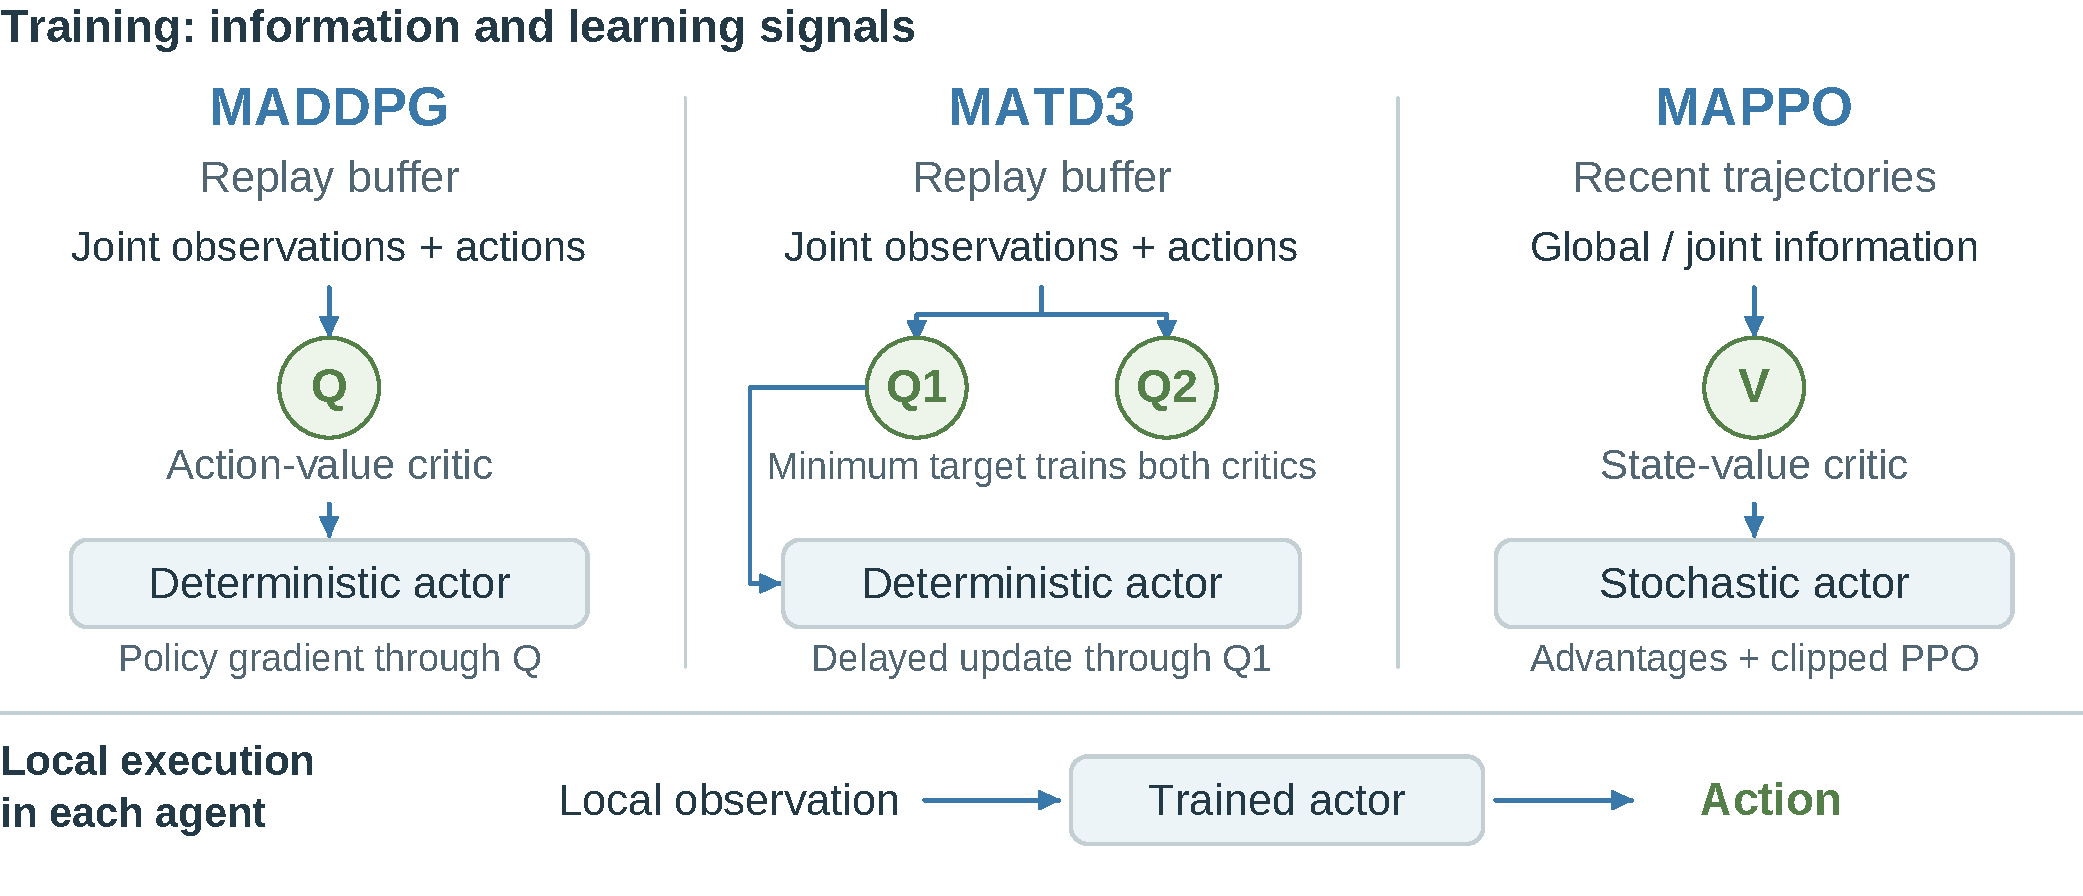
\includegraphics[width=\textwidth]{figures/review-actor-critics.pdf}
\caption{Critic information and actor updates in \gls{maddpg}, \gls{matd3}, and \gls{mappo}, followed by their common local execution pattern. Critic-to-actor arrows indicate learning signals. Original schematic based on \textcite{lowe2017maddpg,ackermann2019matd3,yu2022mappo}.}
\label{fig:ch3-actor-critics}
\end{figure}

\Needspace{6\baselineskip}

\textcite{lowe2017maddpg} introduce \gls{maddpg} with a deterministic actor and a centralised action-value critic for each agent. Joint observations and actions let the critic assess a decision in the context of the others, while training reuses experience from a replay buffer. This distributes action selection across agents, although the critic's joint input grows with the represented population.

\textcite{ackermann2019matd3} develop \gls{matd3} to reduce overestimation in these value estimates, using twin critics, target-action smoothing, and delayed actor updates. The lower target estimate guides critic learning. Their particle and simulated robotic experiments address the reliability of learning among interacting agents. \gls{matd3} retains \gls{maddpg}'s joint-information requirement, so supporting larger populations still depends on how that information is represented and shared.

\textcite{yu2022mappo} evaluate \gls{mappo}, which trains stochastic actors from recent trajectories using a centralised state-value critic and clipped policy updates. The critic supplies advantage estimates, while the clipped objective moderates changes to the policy. Their cooperative benchmarks show that this on-policy alternative can compete with more specialised \gls{marl} methods. Shared policies for homogeneous agents let several agents contribute experience to one learner. Critic inputs, value normalisation, and data reuse also affect learning performance.

Other actor--critic methods address credit assignment and the organisation of updates. \gls{coma} policy gradients compare an agent's action with alternatives while retaining the others' actions \parencite{foerster2018coma}. \gls{happo} and \gls{hatrpo} use sequential updates without requiring parameter sharing \parencite{kuba2022happo}.

\Needspace{5\baselineskip}
\smallskip
\noindent\textbf{Shared learning and value factorisation}\par\nobreak\smallskip
The learning rule alone leaves open how experience and value estimates are organised across the population. One option is to share a policy, so that several agents contribute observations, actions, and outcomes to the same learning process. Each agent then uses that policy with its own observations. \textcite{terry2023sharing} examine parameter sharing among heterogeneous agents, including differences in observation and action spaces. Agent characteristics or identifying information let the common policy distinguish their circumstances. This is relevant to communities whose members make similar decisions, such as charging batteries, but have different demands and storage capacities.

A complementary choice concerns how individual decisions contribute to the value of cooperation. Value factorisation constructs a joint value estimate from smaller components, making that structure explicit. \textcite{rashid2018qmix} introduce a monotonic mixing network that combines individual value estimates into a team value, allowing locally selected greedy actions to agree with the joint choice. For continuous actions, \textcite{peng2021facmac} develop \gls{facmac}, combining a factored critic with policy updates that account for the joint action. Sharing reuses learning across agents, while factorisation organises the joint value being learned. The two choices can support the same controller.

Residential coordination provides an application of this structured learning. \textcite{charbonnier2025rehearsal} apply \gls{facmac} with optimisation-informed learning to communities of up to 30 homes. Their simulations report reduced learning effort and operating costs relative to the compared controllers, with training for the evaluated configurations. The study examines how value decomposition and optimisation guidance contribute to the results. It shows how organising the training procedure can make coordinated residential control more practicable as more homes are considered.

\Needspace{5\baselineskip}
\smallskip
\noindent\textbf{Organising interactions across the population}\par\nobreak\smallskip
Beyond sharing experience and structuring value estimates, methods can simplify the interactions considered by each agent. Mean-field \gls{rl} represents the influence of other agents through an aggregate, such as an average action \parencite{yang2018meanfield}. Localised learning retains interactions within a neighbourhood, with approximation guarantees when the influence of distant agents decays sufficiently rapidly \parencite{qu2020scalable}. These approaches describe the population at different resolutions. In community energy control, an aggregate may describe collective demand, whereas a neighbourhood can retain the relationships between members sharing a local network connection.

Graphs and hierarchies organise these interactions explicitly. \textcite{boehmer2020coordination} factor the team value into individual and pairwise terms on a coordination graph, using message passing to select joint actions. In the feudal multi-agent approach of \textcite{ahilan2019feudal}, managers set subgoals and workers select actions to pursue them. Hierarchy offers a way to separate community allocation from local equipment decisions, provided that the subgoals convey the requirements each level must meet.

Attention learns which information matters within the represented population. \textcite{savino2025attention} use an attention-based central critic with a separate actor for each building. Their CityLearn simulations include districts of up to 73 buildings in California and 100 in Texas, with electrical and domestic-hot-water storage. The reported results improve the trade-off between operating cost and district load variation, connecting selective information use with control across a substantial population.

These methods organise learning for a specified population through shared experience, structured values, and selective coordination. Continued control after members or equipment change also requires suitable observation and action interfaces. Section~\ref{sec:ch3-reconfiguration} examines architectures that accommodate such changes.

\Needspace{9\baselineskip}
\subsection{Architectures for Variable Agent and Resource Configurations}
\label{sec:ch3-reconfiguration}

When members or equipment enter or leave a community, the controller's observations and commands must reflect the resulting configuration. This subsection reviews complementary design choices for accommodating these changes, beginning with set aggregation and attention, followed by entity-to-action mappings, graph representations, and modular reuse.

\Needspace{5\baselineskip}
\smallskip
\noindent\textbf{Set aggregation and attention for entity representation}\par\nobreak\smallskip
Representing resources as separate entities frees their measurements from permanent positions in a fixed input vector. In Deep Sets, \textcite{zaheer2017deepsets} apply a shared transformation to each element, followed by an aggregation independent of element order. The same operations process different numbers of elements. Retaining each resource's representation alongside the pooled summary makes individual circumstances and collective conditions available for control.

Pooling forms a common summary, while attention lets each entity incorporate information from others. The Transformer introduces attention over input representations \parencite{vaswani2017attention}, and the Set Transformer develops it for unordered collections \parencite{lee2019settransformer}. In a \gls{rec}, attention could relate a battery's available capacity to a charging request elsewhere. The supplied attributes and relationships, including resource ownership, determine what the policy can learn from that interaction.

\Needspace{5\baselineskip}
\smallskip
\noindent\textbf{Entity-to-action mappings and action semantics}\par\nobreak\smallskip
Entity representations describe what is present, while the action interface determines which entities receive decisions and what those decisions mean. \gls{updet} connects entity observations to action groups \parencite{hu2021updet}. Contextual entities can inform decisions without requiring actions of their own. StarCraft experiments evaluate transfer between team sizes before and after additional learning. For a \gls{rec}, this distinction separates context such as weather and prices from equipment requiring commands.

An explicit entity interface connects these representations to environment observations and actions. Entity Gym describes entity types and their features, variable collections of instances, and actions associated with acting or target entities. Availability masks restrict which entities and actions can be selected. RogueNet supplies a compatible Transformer policy with encoders shared within each entity type and heads for the declared action spaces. \textcite{symesthompson2025entity} evaluate this combination with \gls{ppo} in simulated cyber defence, including transfer to unseen network sizes. Their experiments concern variation across networks; changes in entity population within an episode are discussed as a further application. This is a close precedent for combining typed entities, variable observations, and resource-associated decisions.

Output queries provide another way to associate decisions with entities. In Perceiver IO, \textcite{jaegle2022perceiver} encode inputs into a latent representation and use queries to request outputs, allowing input and output layouts to vary independently. A resource-specific query could request an equipment command. This is a possible control application of the general-purpose mechanism.

Action meaning introduces a separate requirement when parameters are shared across heterogeneous agents. \textcite{yu2024uas} construct a \gls{uas} that distinguishes actions by their effects and targets, then use availability masks to recover each agent group's policy. An auxiliary prediction loss uses one group's trajectory to predict other groups' policies. The resulting U-\gls{mappo} and U-QMIX methods are evaluated in \gls{smac}. Their relevance is the preservation of different action semantics within shared learning, such as distinguishing an attack from a healing action, rather than treating equal action indices as equivalent. In energy control, this motivates distinguishing commands with different effects even when their numerical representations have the same shape.

\Needspace{5\baselineskip}
\smallskip
\noindent\textbf{Graph representations for changing relationships}\par\nobreak\smallskip
The associations considered so far connect entities to their observations and actions. Graphs also represent relationships among entities, allowing the controller to use the structure of the current configuration. In message-passing neural networks, shared functions update a node using information from neighbouring nodes and their connecting edges \parencite{gilmer2017mpnn}. A community graph can distinguish members from equipment and represent ownership or electrical connections. Adding a battery introduces its node and the relevant relationships; removing a member also removes the associated resources from the active representation. The policy can apply the same message-passing functions to the updated graph. Which relationships are included determines what information can influence each decision.

Changing tasks can also alter the actions available to otherwise familiar agents. \textcite{anil2025mohito} model this setting with task-open Markov games and the MOHITO actor--critic method. Its evolving hypergraph links agents, tasks, and actions, allowing graph-based actors and critics to evaluate the current choices. Simulated ridesharing and wildfire-suppression experiments examine tasks appearing and disappearing during operation. For a \gls{rec}, an arriving vehicle creates a service request, whereas installing a charger changes the equipment available to serve requests. MOHITO provides a precedent for dynamic task--action relations; relating temporary tasks to persistent equipment and community members requires those objects to be distinguished in the energy formulation.

Agent participation introduces another form of variation. The open-teamwork studies of \textcite{rahman2021gpl,koh2025flickerfusion} consider agents entering and leaving, while \textcite{cai2024comat} evaluate unseen team compositions in robot cooperation. These studies complement MOHITO's task changes by examining changes to the agents available to perform the work.

Energy applications connect graph representations to variable participation. \textcite{orfanoudakis2025evgnn} map active charging sessions to commands within the electrical infrastructure, reaching 1,000 charging points with separate training at the evaluated sizes. \textcite{orfanoudakis2026gnndt} instead evaluate a \gls{gnndt} trained for 25 stations on configurations with 5--100 stations without further training. The latter demonstrates reuse across infrastructure sizes, although performance deteriorates towards larger configurations.

Recent methods combine graph structure with cooperative learning or runtime protection. The HetGPS preprint uses shared \gls{marl} policies, a heterogeneous infrastructure graph, and a physical safety filter in simulations with 200--3,218 \glspl{ev}, including transfer and limited adaptation \parencite{wang2026hetgps}. In voltage control, \textcite{jin2026gras} evaluate a shared graph actor--critic with \gls{ac} screening, termed \gls{grasavc}, on an unseen feeder, changes in active inverter participation, and an announced topology change. An updated graph and electrical model support a runtime comparison between the learned command and a droop fallback.

Real-world charging provides an example of managing changing participation through conventional control. \textcite{hermans2024mpc} implement predictive control at an office complex, updating charging allocations as vehicles arrive and depart. Their trial demonstrates this response on operating chargers, complementing the simulated learning-based studies above.

\Needspace{5\baselineskip}
\smallskip
\noindent\textbf{Modular composition and reuse across resource types}\par\nobreak\smallskip
The entity-to-action mappings reviewed above establish which resource receives each decision. Modular composition concerns which learned components can be reused when those resources change. The two choices can be combined, as the type-specific encoders in Entity Gym/RogueNet already illustrate. The studies below develop reuse across bodies, interfaces, and equipment configurations. In Shared Modular Policies, \textcite{huang2020smp} assign shared control modules to robot limbs and exchange information according to the body structure, allowing one policy to control different morphologies. Each module remains responsible for its own actions. For energy systems, this suggests reusable control components associated with batteries, charging points, or other equipment. Their inputs and outputs must reflect the equipment type, since charging a battery and scheduling a flexible appliance involve different decisions and operating requirements.

Modularity can also separate how a system is observed from how it is controlled. \gls{coin} connects specialised perception and action modules through a shared Transformer controller \parencite{luketina2025compositional}. \gls{bc} in a compositional grid-world evaluates held-out combinations of observation, action, and instruction spaces. Further experiments introduce a new observation modality by training its perception module while retaining the controller and action modules. This establishes reuse through recombination of learned interfaces and adaptation of selected components. Its learning setting is imitation rather than cooperative \gls{marl}.

Building2Building provides an energy example, connecting \gls{hvac} measurements and commands through typed graphs and type-specific encoders and decoders \parencite{taboga2026building2building}. Its single-agent \gls{ppo} controller reuses a Transformer policy across building configurations. EnergyPlus experiments evaluate temperature tracking in held-out buildings, with energy cost excluded from the objective.

Software typing and equipment descriptions support integration. The \texttt{marlenv} library provides strongly typed environment records and action-availability masks \parencite{marlenv2026software}. Brick describes equipment, measurement points, and their relationships \parencite{balaji2018brick}. These supply interface structure and resource semantics, while the policy architecture determines how they inform decisions.

The reviewed studies distinguish training for each configuration, applying a policy without further learning, and adapting it to a new setting. The charging transfer results illustrate why these conditions matter when comparing performance across configurations. The following synthesis brings these forms of reuse together with the capabilities of the reviewed architectures.

\subsection{Comparative Analysis and Remaining Questions}
\label{sec:ch3-scalability-gaps}
\label{sec:ch2-gap-rq1}

Table~\ref{tab:ch3-scaling-evidence} summarises the reviewed capabilities, the associated methods, and the settings in which they were evaluated.

\begingroup
\small
\setlength{\tabcolsep}{4pt}
\renewcommand{\arraystretch}{1.10}
\begin{longtable}{@{}>{\raggedright\arraybackslash}p{\dimexpr .22\textwidth-1.333\tabcolsep\relax}>{\raggedright\arraybackslash}p{\dimexpr .45\textwidth-1.333\tabcolsep\relax}>{\raggedright\arraybackslash}p{\dimexpr .33\textwidth-1.334\tabcolsep\relax}@{}}
\caption{Capabilities established by the studies reviewed in Section~\ref{sec:ch3-reconfiguration}.}\label{tab:ch3-scaling-evidence}\\
\toprule
Capability & Methods and references & Evaluation setting\\
\midrule
\endfirsthead
\caption[]{Capabilities established by the studies reviewed in Section~\ref{sec:ch3-reconfiguration} (continued).}\\
\toprule
Capability & Methods and references & Evaluation setting\\
\midrule
\endhead
\midrule
\multicolumn{3}{r}{\emph{Continued on the next page.}}\\
\endfoot
\bottomrule
\endlastfoot
Entity-associated decisions & \gls{updet} and Entity Gym/RogueNet \parencite{hu2021updet,symesthompson2025entity}. & Transfer across game teams and cyber networks.\\
\addlinespace[4pt]
Heterogeneous action meanings & \gls{uas} with U-\gls{mappo} and U-QMIX \parencite{yu2024uas}. & Heterogeneous game actions in \gls{smac}.\\
\addlinespace[4pt]
Changing tasks and choices & MOHITO \parencite{anil2025mohito}. & Tasks appearing and disappearing in simulated ridesharing and wildfire suppression.\\
\addlinespace[4pt]
Reuse of learned modules & Shared Modular Policies, \gls{coin}, and Building2Building \parencite{huang2020smp,luketina2025compositional,taboga2026building2building}. & Robot morphologies, interface combinations, and buildings. \gls{coin} uses imitation and Building2Building uses single-agent \gls{ppo}.\\
\addlinespace[4pt]
Reconfiguration in energy control & \gls{gnndt}, HetGPS, \gls{grasavc}, and predictive charging \parencite{orfanoudakis2026gnndt,wang2026hetgps,jin2026gras,hermans2024mpc}. & Simulated charging networks and inverter control. Real-world charging uses \gls{mpc}.\\
\end{longtable}
\endgroup

The evidence reviewed in this section and summarised in Table~\ref{tab:ch3-scaling-evidence} establishes several foundations for control across changing configurations. \gls{updet} and Entity Gym/RogueNet associate decisions with variable collections of entities, MOHITO updates relationships between agents, tasks, and actions, and Shared Modular Policies and \gls{coin} reuse learned components across different configurations. Graph-based energy controllers also demonstrate transfer across infrastructure sizes and operation under changes in participation. These capabilities provide concrete starting points for investigating how coordination can continue as a community changes.

The condition requiring further investigation combines member entry and departure with equipment additions and removals within members under cooperative \gls{marl} control of a \gls{rec}. Within the reviewed literature, no evaluation was identified that jointly examines these changes. A departing member removes demand and flexibility, while equipment added elsewhere introduces decisions and capacity associated with another member's services. The controller must preserve the associations between members, equipment, service requirements, and executable actions as both levels change. The question is how well existing approaches support this condition, considering community performance, individual service delivery, and computational demand. Performance immediately after reconfiguration must also be distinguished from performance recovered through further learning. This investigation concerns new instances and combinations of recognised equipment types.

A comparison under common operating conditions can establish how far the reviewed capabilities meet these requirements and where adaptations are needed. Differences in available information, action scope, execution protection, and learning resources must be accounted for when interpreting the results. Entity-based decisions, changing task relationships, and reusable modules offer alternative ways to organise this control problem, each with preparation and computational costs to assess. The absence of a joint evaluation motivates this comparison. Whether additional mechanisms are needed, and what they should change, must follow from the limitations observed in that comparison.

\FloatBarrier
\section{Deployability across Heterogeneous Installations}
\label{sec:ch3-deployability}

A controller prepared for one energy community may need new data, local adjustment, and different equipment connections before it can serve another. These activities take time and engineering work, even when the policy can represent the new configuration. Following Section~\ref{sec:intro-lexicon}, deployability concerns the effort needed to prepare, integrate, and maintain useful control. Section~\ref{sec:ch3-scalability} examined the configurations that learning methods and architectures can accommodate. This section is concerned with how much of the preparation for control can be reused across installations.

Section~\ref{sec:ch3-data-prior-knowledge} examines learning from operational records and prior control knowledge. Section~\ref{sec:ch3-transfer} then considers policy reuse, selection, and adaptation, while Section~\ref{sec:ch3-deployment-evidence} examines integrated control systems, from equipment interfaces and operational platforms to controller testing and updates. Section~\ref{sec:ch3-deployability-gaps} compares the evidence and identifies the remaining question about their combined preparation effort.

\subsection{Learning from Available Data and Prior Knowledge}
\label{sec:ch3-data-prior-knowledge}
\label{sec:ch2-experience-literature}

Learning through repeated interaction with an occupied building takes time, and exploratory decisions affect energy use and the services delivered to occupants. Preparation can begin with information already available at the site. Records of earlier operation show how equipment responded to control decisions, while existing rules and predictive models provide knowledge that can guide learning. The review first examines imitation and offline \gls{rl} from these records, then considers guidance from rules and models. It finally turns to community-level learning, where the recorded outcomes depend on decisions made by several agents.

\Needspace{5\baselineskip}
\smallskip
\noindent\textbf{Behaviour cloning and offline reinforcement learning}\par\nobreak\smallskip
\gls{bc} learns to reproduce recorded actions. Offline \gls{rl} also uses their outcomes to seek improved behaviour from a fixed archive. As explained in Section~\ref{sec:ch2-offline}, the difficulty is assessing actions for which that archive provides little evidence. A policy can otherwise favour actions whose estimated value is high because the estimate is unreliable.

Several methods restrict this improvement in different ways. \gls{bcq} generates candidate actions from a model of recorded behaviour and allows bounded adjustments \parencite{fujimoto2019bcq}. \gls{cql} penalises optimistic values for actions insufficiently supported by the data \parencite{kumar2020cql}. \gls{iql} learns values from observed actions and uses them to weight \gls{bc}, avoiding unseen actions in its value-learning updates \parencite{kostrikov2021iql}. These choices control how far learning relies on information beyond the archive.

A simpler combination adds a \gls{bc} penalty to \gls{td3} and normalises the observed states; the resulting method is denoted \acrshort{td3}+\acrshort{bc} \parencite{fujimoto2021td3bc}. Its competitive continuous-control results make it relevant where implementation and tuning effort matter alongside performance. These algorithms supply candidates for learning from energy records. Their general-control benchmarks do not establish a performance ranking for buildings.

Real-world room control illustrates why the application matters. \textcite{liu2022safehvac} extend \gls{bcq} with value regularisation to obtain \gls{bcm}. The study uses a year of operational records and evaluates temperature and airflow control in 15 rooms on three floors, with individual runs lasting approximately one week. \gls{bcm} gives more stable performance than the compared batch-learning alternatives, with a different method ranking from the simulated evaluation. Rule-based comparisons use historical weeks selected for similar outdoor temperatures. The study connects fixed-data learning to real-world execution while showing the importance of the records and comparison conditions.

The controller that collects those records also affects their usefulness. \textcite{nweye2022realworld} initialise policies from rule-based experience before continuing learning in CityLearn. More records from a basic controller can impair performance, whereas a stronger collecting policy supplies better preparation and remains competitive with the learned alternatives. The result distinguishes archive size from useful coverage. It also separates fully offline learning from initialisation intended to shorten subsequent interaction.

\Needspace{5\baselineskip}
\smallskip
\noindent\textbf{Rule-guided learning and model-based preparation}\par\nobreak\smallskip
Existing control knowledge can guide updates as well as generate demonstrations. A rule-guided offline learning method (RUBICON) uses critic estimates over a minibatch to select either recorded behaviour or a rule-based reference for regularising offline actor updates \parencite{liu2023rubicon}. Its online form regularises \gls{td3} using the reference controller. Simulated \gls{hvac} experiments vary climate, data quality, and response uncertainty, showing how rules can supplement uneven experience without requiring equal imitation of every recorded action.

Prior knowledge can also shape the policy itself. Gnu-\gls{rl} combines a differentiable predictive-control structure with imitation-based initialisation and subsequent policy-gradient learning \parencite{chen2020gnurl}. Its conference-room study uses 20 selected historical days for training and 13 for testing, followed by three weeks of real-world airflow control. Temperature tracking improves and cooling demand decreases relative to the existing controller. Residual learning uses established control differently: a learned correction is added to a retained feedback controller, as demonstrated in real-world robotic assembly by \textcite{johannink2019residual}. One approach incorporates planning into the learned policy, while the other preserves a baseline contribution to each action.

Records can instead prepare a model through which a policy learns. In domestic hot-water control, \textcite{recP02} share information across 53 households to support thermal modelling. The field implementation uses a simplified controller, partly to make learning, control, and communication faults easier to diagnose. In a laboratory heating system, \textcite{blad2023laboratory} learn recurrent dynamics from operational data, train a multi-agent controller through that model, and continue learning on the testbed. Conventional control remains active outside the learned operating region. Model-based preparation reduces physical interaction while introducing identification and validation work.

\Needspace{5\baselineskip}
\smallskip
\noindent\textbf{Offline multi-agent learning and joint records}\par\nobreak\smallskip
Community records contain actions whose outcomes depend on other members. Improving each policy independently can produce a joint behaviour poorly represented in the archive. \gls{omar} combines policy-gradient updates with a critic-guided search for better actions \parencite{pan2022omar}. An offline multi-agent method with implicit global-to-local value regularisation (OMIGA) derives local value regularisation from a global regularised objective and combines it with learning from observed actions \parencite{wang2023omiga}. Their multi-agent locomotion, particle, and StarCraft evaluations provide approaches to offline coordination. Community application requires records that preserve the relationship between local actions, shared conditions, and outcomes.

These learning routes need more than meter readings. Policy learning requires decision-time observations, executed actions, and information from which the objective can be reconstructed. Model learning requires data that reveal the relevant dynamics. Data access, alignment, and interpretation therefore contribute to preparation effort. Protection of the eventual actions is considered separately in Section~\ref{sec:ch3-safety}. The next subsection examines how much of a prepared policy can be reused at another installation.

\subsection{Policy Reuse and Adaptation across Installations}
\label{sec:ch3-transfer}

Once a policy has been prepared, its use at another installation offers a way to share that initial investment. Two homes may have similar batteries but different demand patterns, while buildings with comparable heating needs may use different equipment. Reuse therefore depends on both the behaviour learned and the observations and actions available at the new site. A policy may be applied directly, selected from a suitable group, or adapted through local learning. The review examines policy transfer, preparation shared across groups, and adaptation to different interfaces, distinguishing reusable work from the preparation still required at each installation.

\Needspace{5\baselineskip}
\smallskip
\noindent\textbf{Policy transfer and local action models}\par\nobreak\smallskip
Residential batteries provide a direct example of parameter transfer. MERLIN evaluates policy exchange among independent controllers using measured profiles from 17 zero-net-energy homes in CityLearn \parencite{nweye2023merlin}. A source policy receives a further simulated training episode at the target. Reuse can approach locally trained performance with fewer target episodes, although the outcome depends on the source building and performance indicator. Selecting a useful source is therefore part of preparation. Both battery operation and adaptation are simulated.

Training across several sources can spread that initial investment. \textcite{madahi2024multisource} prepare a shared battery policy from 90 Belgian households and adapt its final layer to ten unseen households. Common preparation uses 40,000 episodes, followed by 100 adaptation episodes per target. All households share the battery model and action interface, and evaluation uses April 2023 data. The study demonstrates reduced target learning under different consumption and generation profiles. Reporting source training separately shows what must be reused for that reduction to be worthwhile.

A local model can handle installation differences while retaining a common decision policy. \textcite{xu2020oneformany} separate an \gls{hvac} front-end network from an inverse building model that maps its decisions to equipment actions. The local model is fitted through supervised learning using approximately two weeks of operation under an existing or simple on--off controller. Simulated transfers vary buildings, equipment, and climate, with outcomes depending partly on the direction of climate transfer. This approach shifts target preparation from additional \gls{rl} towards supervised identification.

\Needspace{5\baselineskip}
\smallskip
\noindent\textbf{Cohorts, meta-learning, and federated preparation}\par\nobreak\smallskip
Another route is to select an existing policy for a group of similar installations, or cohort. \textcite{zangato2025policymapping} group buildings by non-shiftable demand and assign three groups to shared policies in CityLearn. Classification from one week of observations agrees with annual-record grouping in their dataset. Cost results improve, while carbon results are more mixed. This provides a way to select behaviour from short records instead of training a separate policy for each new member.

Grouping by behaviour complements the interface compatibility discussed in Section~\ref{sec:ch3-scalability}. Two homes may expose identical battery actions but have different demand patterns. Similar demand, in turn, does not ensure equivalent equipment actions. Policy assignment therefore needs both a compatible interface and evidence that the selected behaviour suits the target. Unfamiliar profiles may call for reassignment or adaptation.

Meta-learning prepares a policy specifically for such adaptation. MetaEMS learns an initialisation through building-level and group-level updates before adapting to target buildings \parencite{zhang2025metaems}. CityLearn experiments separate source and target buildings within four climate zones and report improvements over the compared initialisation and control methods. Target interaction remains part of the procedure, but the shared preparation is organised to make those updates effective.

Federated learning allows sites to share preparation while retaining their operational records. \textcite{hagstrom2025federatedhvac} exchange model updates between \gls{sac} controllers for a simulated two-zone data centre under different climates, including an unseen evaluation climate. Learning and generalisation improve under selected optimisation and aggregation choices, with a trade-off between early comfort violations and final performance. Satisfactory behaviour takes three to 24 simulated weeks, depending on the configuration. Sharing updates thus changes data management as well as learning, while the required interaction remains consequential for real-world use.

\Needspace{5\baselineskip}
\smallskip
\noindent\textbf{Heterogeneous interfaces and real-world transfer}\par\nobreak\smallskip
The preceding approaches reuse compatible policy structures or provide a local mapping. When observation spaces differ, the policy itself may need modification. \textcite{coraci2024heterogeneous} combine model slicing, imitation, and fine-tuning to transfer controllers with different observations and reward formulations. Their simulated cases retain chiller and thermal-storage control, while \gls{pv} and battery systems use rules. Transfer improves on rule-based and initially untrained online controllers, although target-specific simulation training can retain an advantage. Interface adaptation and behavioural adaptation therefore involve distinct work.

Real-world transfer also requires model calibration and actuation access. In HiLo, \textcite{coraci2025hilo} transfer control between two offices in one building using a calibrated digital twin, 14 days of target records, and online fine-tuning. Matched controller comparisons use the twin, and two days affected by an equipment-mode change are excluded from the heating comparison. The trial establishes physical policy reuse alongside the local data and modelling needed to support it.

Table~\ref{tab:ch3-deployability-methods} brings together the preparation mechanisms in Sections~\ref{sec:ch3-data-prior-knowledge} and~\ref{sec:ch3-transfer}. Its rows distinguish what can be reused from what a target still needs. These routes allow compatible installations to receive a policy through selection, local fitting, or adaptation, with different demands on data and training.

\begin{table}[!htbp]
\centering
\caption{Mechanisms for reducing controller preparation and the work retained at a target installation.}
\label{tab:ch3-deployability-methods}
\small
\setlength{\tabcolsep}{4pt}
\renewcommand{\arraystretch}{1.12}
\begin{tabularx}{\textwidth}{@{}>{\raggedright\arraybackslash}p{0.24\textwidth}>{\raggedright\arraybackslash}X>{\raggedright\arraybackslash}X@{}}
\toprule
Mechanism & Reusable preparation & Target requirements\\
\midrule
Offline learning and imitation & Recorded behaviour and its outcomes; trained policy or initialisation. & Action-labelled records, coverage assessment, and validation of the resulting behaviour.\\
\addlinespace
Model-based preparation & Predictive structure, shared identification data, or a simulation workflow. & Local identification or calibration where needed; validation against operation.\\
\addlinespace
Parameter transfer and fine-tuning & Source policy or representation. & Compatible inputs and actions; target data and the updates used for adaptation.\\
\addlinespace
Transferable policy with local model & Common decision policy. & Supervised fitting of an installation-specific action mapping.\\
\addlinespace
Cohorts and policy mapping & Policies shared by compatible groups. & Group assignment, interface checks, and assessment of unfamiliar profiles.\\
\addlinespace
Meta-learning & Initialisation trained for adaptation across related tasks. & Target experience and adaptation steps.\\
\addlinespace
Federated learning & Knowledge exchanged through model updates. & Local learning data, compatible models, and aggregation infrastructure.\\
\bottomrule
\end{tabularx}
\end{table}

Reusing learned behaviour is one part of commissioning. The installation must also supply the expected observations and accept the resulting commands. The next subsection examines how software and equipment interfaces make that connection reusable.

\subsection{System Integration and Controller Lifecycle}
\label{sec:ch3-deployment-evidence}

Putting a prepared policy into operation requires a working connection between measurements, decisions, and equipment commands. A battery may report through a local gateway while a heat pump uses a manufacturer's service, so the control system must bring these interfaces together with consistent meanings, units, and timing. The same connections must support subsequent controller versions as they are tested and introduced into operation. The review follows this progression from device adapters and semantic descriptions to integrated energy platforms, then examines the infrastructure for testing, deployment, and controller updates.

\Needspace{5\baselineskip}
\smallskip
\noindent\textbf{Device adapters and semantic descriptions}\par\nobreak\smallskip
Protocol abstraction separates device communication from application logic. The \gls{bemoss} platform places application and data-management functions above VOLTTRON communication services \parencite{khamphanchai2014bemoss}. Device discovery and control agents expose supported interfaces, including \gls{bacnet} and Modbus. Its architecture and laboratory testbed show how applications can share communication functions. A new device may need an adapter, which can subsequently serve several applications.

Semantic descriptions specify what those connected data mean. Brick represents equipment, measurement points, and relationships so that applications can find data by their roles \parencite{balaji2018brick}. Its evaluation covers six commercial buildings with more than 17,700 points and eight applications, four operating across all six buildings. Mortar combines records from 90 buildings and evaluates 11 portable analytics applications whose declared requirements determine usable sites \parencite{fierro2018mortar}. For learned control, the same principle can support consistent observations assembled from different site descriptions.

BuildingMOTIF checks whether a site's semantic description supplies the information an application needs \parencite{fierro2022buildingmotif}. Templates reuse equipment structures, and validation identifies missing properties or relationships. Evaluation uses 46 existing Brick models and control-sequence metadata for a reference building, supporting incremental preparation of the descriptions needed by each application.

\Needspace{5\baselineskip}
\smallskip
\noindent\textbf{Integrated control platforms and operational services}\par\nobreak\smallskip
Energy platforms connect these interfaces to forecasting, scheduling, and actuation. \textcite{jelic2025islands} join gateways, time-series and semantic storage, forecasts, and scheduling in a cloud platform for island communities. Schedules become device commands, and acknowledgements return to the platform. Electrical control is evaluated in La Graciosa, with thermal applications also supported in participating communities. The pilot provides evidence of an operating acquisition-to-command chain. Comparisons across different periods make it harder to attribute energy differences to the platform alone.

The occupied-building CIRLEM deployment introduced in Section~\ref{sec:ch3-physical-deployment} makes site integration explicit. Its interoperability and coupling mechanisms translate names, types, and units between the controller and building-management system \parencite{hosseini2026cirlem}. Separating the control service from local point mappings identifies which connections can be reused and which must be configured at another site.

An \gls{rl} economiser recommendation service illustrates operation at a larger scale. \textcite{cui2023economizer} report more than 10,000 rooftop units across over 200 sites, supported by Brick-based standardisation, time-series storage, and hourly cloud inference. One policy is trained per site and shared by its units, with quarterly retraining. Operators validate and enter recommended setpoints because security and trust requirements limit automation. Online performance results are withheld, and expected savings come from simulation. The evidence establishes service organisation and scale while identifying the human work retained in operation.

\Needspace{5\baselineskip}
\smallskip
\noindent\textbf{Testing, deployment, and controller updates}\par\nobreak\smallskip
Once a controller is connected, subsequent versions need repeatable assessment and execution. The \gls{boptest} supplies simulation cases, a common interface, and performance indicators for comparing control changes \parencite{blum2021boptest}. KubeVOLTTRON explores container orchestration for distributing VOLTTRON services \parencite{kempf2022kubevolttron}. These address complementary tasks: testing behaviour under controlled conditions and reproducing service execution. Each installation still needs suitable models, data connections, and command access.

\gls{rlops}, developed for telecommunications, connects data preparation, training, testing, deployment, and monitoring \parencite{li2022rlops}. Its relevance to energy control is the association between model versions, data processing, and evaluation results as controllers change. The economiser service provides an energy example of scheduled retraining, while the building and community platforms establish physical integration. Accepting an update, coordinating policy versions, and restoring a previous controller remain application-specific responsibilities.

Adapters, semantic descriptions, testing environments, and deployment services reduce different parts of commissioning and maintenance. Their connection matters because the observations and commands used in preparation must retain their meaning in operation. The following comparison brings this integration effort together with the data and adaptation requirements reviewed above.

\subsection{Comparative Analysis and Remaining Questions}
\label{sec:ch3-deployability-gaps}
\label{sec:ch2-gap-rq2}

Deployability depends on the combined effort of preparation, training and adaptation, integration, and maintenance across the controller lifecycle, following Section~\ref{sec:intro-lexicon}. Table~\ref{tab:ch3-deployability-comparison} summarises the reviewed approaches, the associated studies, and their evaluation settings.

\begingroup
\small
\setlength{\tabcolsep}{3.5pt}
\renewcommand{\arraystretch}{1.08}
\begin{longtable}{@{}>{\raggedright\arraybackslash}p{\dimexpr .23\textwidth-1.333\tabcolsep\relax}>{\raggedright\arraybackslash}p{\dimexpr .42\textwidth-1.333\tabcolsep\relax}>{\raggedright\arraybackslash}p{\dimexpr .35\textwidth-1.334\tabcolsep\relax}@{}}
\caption{Evaluation settings for controller preparation, reuse, and integration.}\label{tab:ch3-deployability-comparison}\\
\toprule
Approach & Studies and references & Evaluation setting\\
\midrule
\endfirsthead
\caption[]{Evaluation settings for controller preparation, reuse, and integration (continued).}\\
\toprule
Approach & Studies and references & Evaluation setting\\
\midrule
\endhead
\midrule
\multicolumn{3}{r}{\emph{Continued on the next page.}}\\
\endfoot
\bottomrule
\endlastfoot
Learning from operational records & \gls{bcm} and Gnu-\gls{rl} \parencite{liu2022safehvac,chen2020gnurl}. & Real-world \gls{hvac} control in a 15-room study and a conference room.\\
\addlinespace[4pt]
Policy transfer and selection & MERLIN, multi-source transfer, and cohort policy mapping \parencite{nweye2023merlin,madahi2024multisource,zangato2025policymapping}. & Simulated residential batteries with measured demand profiles.\\
\addlinespace[4pt]
Policy transfer in operation & HiLo \parencite{coraci2025hilo}. & Two real offices, supported by a calibrated digital twin and local fine-tuning.\\
\addlinespace[4pt]
Semantic application reuse & Brick, Mortar, and BuildingMOTIF \parencite{balaji2018brick,fierro2018mortar,fierro2022buildingmotif}. & Multi-building analytics and metadata validation.\\
\addlinespace[4pt]
Integrated energy control & Island-community platform and CIRLEM \parencite{jelic2025islands,hosseini2026cirlem}. & Operating community and building systems linking measurements to commands.\\
\addlinespace[4pt]
Controller services and updates & Economiser recommendation service \parencite{cui2023economizer}. & More than 200 sites, with quarterly retraining and operator-applied recommendations.\\
\end{longtable}
\endgroup

The studies brought together in Table~\ref{tab:ch3-deployability-comparison} establish several ways to prepare and deploy controllers, from learning with existing records to reusing policies and connecting them to equipment. Their results include real-world control and services operating across many sites. The reviewed literature, however, does not provide a common assessment of data preparation, policy adaptation, equipment integration, and controller updates together for communities with different member and resource configurations. A reduction in target training may nevertheless depend on a calibrated model, prepared metadata, or equipment connections established in advance. These activities contribute to the effort of deployment even when they fall outside the learning procedure being evaluated.

That effort depends on what changes between installations. A compatible member may need policy assignment and data mapping, whereas a different thermal response may require local identification or fine-tuning. A new equipment interface can require an adapter as well as changes to the policy. Some of this work can support several installations, while local calibration, validation, and subsequent updates may recur at each site. Comparing the alternatives therefore requires relating retained performance to both shared preparation and repeated local effort, including unsuccessful transfers. The gap concerns how far these activities can be reused together while preserving community performance and individual services across heterogeneous installations.


\FloatBarrier
\section{Physical and Operational Safety}
\label{sec:ch3-safety}

A charging command must respect the equipment's rating and the available connection capacity while leaving enough time to deliver the energy required at departure. Other resources may depend on that same capacity. Following Section~\ref{sec:intro-lexicon}, safety concerns these physical, electrical, and service constraints on applied actions and resulting states. Connecting a controller to equipment, as discussed in Section~\ref{sec:ch3-deployability}, makes their enforcement part of operation.

Section~\ref{sec:ch3-constraint-representation} examines how constraints enter learning and planning. Section~\ref{sec:ch3-action-protection} reviews mechanisms that adjust or replace proposed actions, and Section~\ref{sec:ch3-coordinated-service} considers shared limits and service commitments over time. Section~\ref{sec:ch3-safety-gaps} compares the evidence and identifies the remaining question about their combined effects on community services.

\subsection{Constraint Representation in Learning and Control}
\label{sec:ch3-constraint-representation}

A power rating limits an instantaneous action, whereas a departure request links several decisions to a future outcome. These requirements can enter the reward, constrain policy improvement, or restrict a planned trajectory. Building on Section~\ref{sec:ch2-constrained-foundations}, the discussion first considers learning objectives and then explicit models that connect present decisions to admissible future states.

\Needspace{5\baselineskip}
\smallskip
\noindent\textbf{Reward penalties, cost budgets, and risk criteria}\par\nobreak\smallskip
Reward penalties make undesirable outcomes costly during learning. Exceeding a power threshold or leaving energy undelivered can reduce the reward alongside the benefit of economical operation. The weights determine the trade-off that the policy learns. Constrained learning instead separates the performance objective from an admissible cost budget, making that requirement explicit in policy improvement \parencite{achiam2017cpo,gu2023safemarl}.

\gls{cpo} uses performance and constraint-cost bounds to construct updates within a trust region \parencite{achiam2017cpo}. Its constraint concerns an expected accumulated cost. Lagrangian methods increase the pressure on costs that exceed their budgets through adjustable multipliers. In cooperative learning, \textcite{gu2023safemarl} account for successive changes in the joint policy through \gls{macpo} and \gls{mappo}-Lagrangian. Their simulated multi-robot experiments provide methods for learning with individual or shared budgets while retaining interactions between agents.

Risk criteria address outcomes that an average can conceal. A chance constraint limits the probability of a specified event, while \gls{cvar} describes the costly tail of an outcome distribution. \textcite{chow2018risk} develop policy-gradient and actor--critic methods for percentile-risk criteria. For energy control, defining the event and horizon determines whether the criterion concerns one departure, repeated comfort losses, or an entire operating period. Penalties, expected-cost budgets, and risk criteria therefore express different requirements.

\Needspace{5\baselineskip}
\smallskip
\noindent\textbf{Predictive constraints and model-based verification}\par\nobreak\smallskip
Explicit optimisation places constraints on the decisions being computed. \gls{mpc} plans from the current state and forecasts, applies the first decision, and then replans. A charging formulation can impose power limits throughout the horizon and sufficient energy at departure. Real-world charging provides an operational example \parencite{hermans2024mpc}, while predictive safety filters use related optimisation to check proposals from learned controllers \parencite{wabersich2021predictive}.

Uncertainty determines which future conditions that plan covers. Nominal planning uses an anticipated trajectory, robust formulations impose requirements over a specified disturbance range, and probabilistic formulations associate compliance with a stated probability. Reserving capacity against more possible demand protects a wider range of conditions while reducing the flexibility available for economical scheduling \parencite{wabersich2021predictive,muntwiler2020distributed}.

Learning can also supply proposals for model-based verification. \textcite{zhang2021safemicrogrids} combine supervised multi-agent policy learning, model-derived gradients, and consensus on shared constraint variables. A power-flow calculation checks actions, and backtracking tightens bounds and updates policy parameters when violations are found. Simulations of five interconnected microgrids demonstrate the combination for equipment and network constraints. The resulting decisions depend on both learning and verification. The next subsection examines how such checks modify the commands that reach equipment.

\subsection{Action Protection and Supervisory Enforcement}
\label{sec:ch3-action-protection}
\label{sec:ch2-safety-literature}

A proposed action can be accepted, adjusted, or replaced. Protection mechanisms differ in how they find an admissible alternative and how far ahead they examine its effects. The review separates restrictions on policy outputs, checks of continued admissibility, and supervision using an established controller.

\Needspace{5\baselineskip}
\smallskip
\noindent\textbf{Admissible outputs and projection layers}\par\nobreak\smallskip
Simple restrictions define available actions: a mask can remove charging when a vehicle is absent, and a bounded output can respect its charger's rating. State-dependent constructions go further. \textcite{tabas2022efficient} map neural-policy outputs into actions that preserve a prepared robustly controlled invariant set. Their frequency-control simulations use a closed-form mapping whose protection depends on the supporting model, controller, and set.

Projection preserves a proposal as closely as possible while imposing constraints. \textcite{dalal2018safe} learn a local approximation of how actions affect a safety signal, then use it to correct continuous-control decisions. Their analytical solution assumes feasibility and at most one active constraint. The approximation defines what the correction protects, making its accuracy central to the mechanism.

An optimisation layer can also connect correction to learning. \textcite{agrawal2019differentiable} differentiate through convex programmes so that upstream network parameters can be trained through the constrained solution. Gnu-\gls{rl} provides a physical example of a differentiable \gls{mpc} policy with bounded airflow actions and temperature tracking in its objective \parencite{chen2020gnurl}. Its three-week conference-room experiment demonstrates structured commands for real equipment, with action bounds and thermal performance playing distinct roles.

\Needspace{5\baselineskip}
\smallskip
\noindent\textbf{Predictive filters, barrier functions, and shields}\par\nobreak\smallskip
Predictive protection checks whether an action admits a suitable continuation. \textcite{wabersich2021predictive} search for a trajectory satisfying state and input constraints and reaching a terminal set with a safe controller. When a new full-horizon plan is unavailable, a shortened-horizon route retains the previous certification. The probability of satisfying the constraints depends on initial feasibility, model-error assumptions, and the terminal construction. The check therefore concerns both the present command and the ability to continue operating within the specified constraints.

\glspl{cbf} express continued admissibility through a condition on state evolution. \textcite{ames2017cbf} place this condition in a quadratic programme that combines a control objective with preservation of a specified set. Forward invariance means that a system starting in that set remains there under the stated dynamics and control conditions. Applying this principle to sampled energy control requires appropriate treatment of response times and actuation limits.

Formal shields instead use a permitted-behaviour specification and a system abstraction to replace inadmissible proposals. \textcite{elsayedaly2021shielding} develop centralised shielding of joint actions and factored shielding over subsets of agents. Their simulated multi-agent experiments demonstrate protection during learning and improved scalability through factorisation. The abstraction and consistency between local shields determine the joint property being preserved.

\Needspace{5\baselineskip}
\smallskip
\noindent\textbf{Supervisory switching and reference controllers}\par\nobreak\smallskip
Supervision can retain an established controller alongside the learned one. The Neural Simplex Architecture allows learned control while recovery by a baseline remains possible and switches before that option is lost \parencite{phan2020neuralsimplex}. It also supports learning after intervention. The switching condition matters because the fallback controller protects a defined operating region.

Physical heating illustrates this division of responsibility. \textcite{blad2023laboratory} control the supply and valves of a two-zone underfloor-heating system with \gls{marl} and temperature-based supervisors. Intervention also affects the learning reward. Measured temperatures describe the delivered service, while heat-pump electricity cost is modelled because the testbed uses a different heat source. The experiment establishes learned coordination alongside conventional protection on physical equipment.

A supervisor can alternatively compare candidate actions. In graph-based voltage control, \textcite{jin2026gras} use an \gls{ac} power-flow model to evaluate the learned proposal and a droop-control candidate at the same state. The selector applies the action with lower modelled voltage risk. Simulations report reduced voltage exposure together with residual violations. This is a relative selection criterion, distinct from preserving a certified recovery region.

Table~\ref{tab:ch3-safety-mechanisms} compares the requirements and properties of these mechanisms with their information needs. It includes the learning formulations in Section~\ref{sec:ch3-constraint-representation}, making explicit the distinction between guiding policy updates and enforcing conditions during execution.

\begingroup
\fontsize{9.5}{11.3}\selectfont
\setlength{\tabcolsep}{3.5pt}
\renewcommand{\arraystretch}{1.04}
\begin{longtable}{@{}>{\raggedright\arraybackslash}p{\dimexpr .23\textwidth-1.5\tabcolsep\relax}>{\raggedright\arraybackslash}p{\dimexpr .27\textwidth-1.5\tabcolsep\relax}>{\raggedright\arraybackslash}p{\dimexpr .26\textwidth-1.5\tabcolsep\relax}>{\raggedright\arraybackslash}p{\dimexpr .24\textwidth-1.5\tabcolsep\relax}@{}}
\caption{Mechanisms for representing and enforcing control constraints.}\label{tab:ch3-safety-mechanisms}\\
\toprule
Mechanism & Requirement represented & Property or role & Information and preparation\\
\midrule
\endfirsthead
\caption[]{Mechanisms for representing and enforcing control constraints (continued).}\\
\toprule
Mechanism & Requirement represented & Property or role & Information and preparation\\
\midrule
\endhead
\midrule
\multicolumn{4}{r}{\emph{Continued on the next page.}}\\
\endfoot
\bottomrule
\endlastfoot
Penalties and constrained policy learning \parencite{achiam2017cpo,gu2023safemarl} & State, action, or accumulated costs. & Incentives or expected-cost budgets guide policy improvement. & Costs, budgets, experience, and update conditions.\\
\addlinespace[3pt]
Risk-constrained learning \parencite{chow2018risk} & Event probability or the tail of accumulated cost. & A specified probabilistic or risk criterion. & Event, horizon, probability model, and risk threshold.\\
\addlinespace[3pt]
Admissible output construction \parencite{tabas2022efficient} & Actions preserving a prepared invariant set. & Constraint satisfaction in the certified domain. & Dynamics, disturbance bounds, and invariant set.\\
\addlinespace[3pt]
Projection and optimisation layers \parencite{dalal2018safe,agrawal2019differentiable} & Conditions defining an admissible action or plan. & Correction relative to an explicit constraint model. & Constraint model, feasibility, and numerical accuracy.\\
\addlinespace[3pt]
Predictive safety filtering \parencite{wabersich2021predictive} & Current action and a continuation to a safe terminal set. & Continued compliance under feasibility and uncertainty assumptions. & Dynamics, uncertainty bounds, terminal controller, and optimisation.\\
\addlinespace[3pt]
Barrier-based control \parencite{ames2017cbf} & A condition preserving an admissible state set. & Forward invariance under the stated dynamics and control conditions. & Barrier, state, actuation limits, and sampling conditions.\\
\addlinespace[3pt]
Centralised or factored shielding \parencite{elsayedaly2021shielding} & A formal safety specification over joint behaviour. & Adherence to the specification within the system abstraction. & Abstraction, shield synthesis, and consistent local composition.\\
\addlinespace[3pt]
Supervisory switching \parencite{phan2020neuralsimplex,jin2026gras} & Recoverability by a baseline, or relative risk of candidate actions. & Recovery-region protection or lower-risk selection. & Baseline, switching condition, and state or model evaluation.\\
\end{longtable}
\endgroup

The next subsection examines how shared physical limits and future service requirements affect protection across resources.

\subsection{Coordinated Physical Limits and Service Feasibility}
\label{sec:ch3-safety-applications}
\label{sec:ch3-coordinated-service}

The vehicle in Section~\ref{sec:ch2-rec-flexibility} arrives at 18:00 with 30\% \gls{soc} and needs 80\% by 08:00. An admissible charging power now may still leave too little time to meet that request. This subsection examines how predictive protection preserves future options, how shared capacity couples local decisions, and how interventions affect delivered service.

\Needspace{5\baselineskip}
\smallskip
\noindent\textbf{Predictive service constraints and intervention feedback}\par\nobreak\smallskip
A predictive constraint can require departure energy while respecting power and storage limits over the remaining intervals. Thermal control has a similar temporal relationship because current heating affects later comfort. \textcite{markgraf2023safedr} use shrinking-horizon \gls{mpc} filters for simulated households with batteries and air conditioning. Each filter imposes local temperature, power, and storage requirements, including terminal battery charge, with bounded forecast errors represented in the constraints.

Their five-household study also makes intervention visible to learning through a penalty proportional to the correction. The selected \gls{mappo} models require 48 corrections with this penalty and 446 without it \parencite{markgraf2023safedr}. Both variants retain the filter. The comparison isolates the benefit of teaching the policy to request fewer corrections while preserving the same protection mechanism.

\Needspace{5\baselineskip}
\smallskip
\noindent\textbf{Shared limits and distributed predictive protection}\par\nobreak\smallskip
Individually feasible schedules may conflict when two vehicles rely on the same connection headroom. As established in Section~\ref{sec:ch2-rec-members}, the relevant limit follows the physical site, phase, feeder, or transformer. Markgraf and Althoff's filters protect uncoupled household constraints, with transformer capacity identified as an extension. Joint protection instead considers combined actions, while hierarchical control can allocate compatible capacity budgets to local controllers.

Distributed predictive certification formalises this coordination. \textcite{muntwiler2020distributed} construct local safety problems for coupled linear systems with bounded disturbances. Neighbours coordinate admissible trajectories and uncertainty bounds using a structured terminal set. In energy control, \textcite{tao2025distributed} combine local \gls{rl} with distributed \gls{mpc} checkers for two interconnected microgrids. Their subsecond frequency-control simulations provide an electrical example of coordinated state and input protection.

CommonPower assigns control responsibilities to resource groups and balancing assets managed by an operator \parencite{eichelbeck2026commonpower}. Symbolic component models support optimisation and safeguards for learned actions. Building experiments combine a heat pump and battery under uncertain forecasts and different learning arrangements. Component constraints receive robust treatment, while power-flow constraints apply to the nominal trajectory. This distinction identifies which uncertainty each level of protection covers.

\Needspace{5\baselineskip}
\smallskip
\noindent\textbf{Intervention order and delivered service}\par\nobreak\smallskip
Multiple safeguards can change the same command in different ways. HetGPS first applies voltage correction and then a mapping for availability, \gls{soc}, and departure rules \parencite{wang2026hetgps}. The second step can alter the electrically corrected action, for example by increasing charging near departure. Simulations across 200--3,218 \glspl{ev} report reduced voltage violations and departure outcomes assessed with a specified \gls{soc} tolerance. Service mapping remains active in all compared variants, so the voltage-filter comparison measures its added effect within an already supervised charging system.

This interaction connects instantaneous protection to future allocation. A projection addresses the present electrical condition, whereas predictive control can also reserve capacity for later obligations. Coordinated capacity budgets provide another way for local schedules to respect arrivals, deadlines, and competing demand. The predictive and distributed mechanisms above supply approaches to that problem, with the resulting service depending on the allocation across participants.

Physical charging reveals additional effects of execution. In the \gls{mpc} study of \textcite{hermans2024mpc}, lower-level allocation and pausing required practical adjustments because two vehicles had difficulties with paused sessions. Average recorded energy per session also differed between comparison periods. These observations accompany the reported peak reduction and show why individual delivery matters alongside aggregate outcomes.

Interpreting a service deficit requires knowing whether the request was feasible. Repeated postponement can make an initially achievable departure target impossible, while another request may exceed available time or capacity on arrival. The former concerns control decisions during service. The latter requires admission, revised commitments, or explicit priorities. This distinction helps compare protection methods without attributing every deficit to the same cause. The final comparison brings together their enforcement scope and the services evaluated.

\subsection{Comparative Analysis and Remaining Questions}
\label{sec:ch3-safety-gaps}
\label{sec:ch2-gap-rq3}

The reviewed methods connect constraint-aware learning, execution protection, and coordinated service in different ways. A policy may learn to request fewer corrections, while a filter enforces its constraint model and conventional equipment control provides further protection. Table~\ref{tab:ch3-safety-evidence} compares these roles in energy applications, retaining the service conditions and the distinction between simulation and real-world operation. The batch-learning and real-world deployment settings are introduced in Sections~\ref{sec:ch3-data-prior-knowledge} and~\ref{sec:ch3-physical-deployment}.

\begingroup
\small
\setlength{\tabcolsep}{3.5pt}
\renewcommand{\arraystretch}{1.06}
\begin{longtable}{@{}>{\raggedright\arraybackslash}p{\dimexpr .21\textwidth-1.5\tabcolsep\relax}>{\raggedright\arraybackslash}p{\dimexpr .28\textwidth-1.5\tabcolsep\relax}>{\raggedright\arraybackslash}p{\dimexpr .23\textwidth-1.5\tabcolsep\relax}>{\raggedright\arraybackslash}p{\dimexpr .28\textwidth-1.5\tabcolsep\relax}@{}}
\caption{Energy-control evidence for physical protection and service delivery.}\label{tab:ch3-safety-evidence}\\
\toprule
Study and setting & Enforcement mechanism & Demonstrated capability & Service or evaluation condition\\
\midrule
\endfirsthead
\caption[]{Energy-control evidence for physical protection and service delivery (continued).}\\
\toprule
Study and setting & Enforcement mechanism & Demonstrated capability & Service or evaluation condition\\
\midrule
\endhead
\midrule
\multicolumn{4}{r}{\emph{Continued on the next page.}}\\
\endfoot
\bottomrule
\endlastfoot
Interconnected microgrids; simulation \parencite{zhang2021safemicrogrids} & Supervised neural policy learning, shared constraint variables, power-flow checking, backtracking. & Coordination of equipment and network constraints in five microgrids. & Applied decisions depend on both the learned policy and model-based verification.\\
\addlinespace[3pt]
Household \gls{dr}; simulation \parencite{markgraf2023safedr} & Local predictive filters and optional intervention penalty during \gls{marl} training. & Protection of battery, power, and thermal constraints over a shrinking horizon. & Terminal battery requirement; uncoupled household constraints. Both learning variants retain protection.\\
\addlinespace[3pt]
Building and grid control; simulation \parencite{eichelbeck2026commonpower} & Symbolic models, predictive safeguards, resource groups and balancing assets. & Robust component protection and comparisons of learned controllers. & Heat-pump and battery case; nominal network constraints. The separate annual network case uses central optimisation.\\
\addlinespace[3pt]
\gls{ev} charging; simulation, preprint \parencite{wang2026hetgps} & Graph \gls{marl}, voltage correction, and subsequent service mapping. & Reduced voltage violations across 200--3,218 \glspl{ev}. & Availability and departure rules active in all variants; final actions determine electrical and service outcomes.\\
\addlinespace[3pt]
Voltage control; simulation \parencite{jin2026gras} & \gls{ac}-model comparison of a graph-policy proposal with droop control. & Lower voltage exposure through candidate selection. & Relative one-step risk criterion; residual voltage violations reported.\\
\addlinespace[3pt]
Microgrid frequency control; simulation \parencite{tao2025distributed} & Local \gls{rl} with distributed \gls{mpc} checking and backup control. & Coordinated state and input protection for two coupled microgrids. & Bounded coupling and disturbance assumptions; subsecond frequency-control task.\\
\addlinespace[3pt]
Conference-room \gls{hvac}; real-world operation \parencite{chen2020gnurl} & Differentiable \gls{mpc} policy with action bounds. & Learned airflow control and improved temperature tracking over three weeks. & Thermal tracking enters the objective; comparison with existing control.\\
\addlinespace[3pt]
Occupied-building \gls{hvac}; real-world operation \parencite{liu2022safehvac} & Batch \gls{rl} with regularised policy learning and a defined action space. & Control of room temperature and airflow from recorded experience. & Empirical comfort assessment; approximately week-long algorithm trials and historical reference periods.\\
\addlinespace[3pt]
Two-zone heating; physical laboratory \parencite{blad2023laboratory} & \gls{marl} supply and valve control with temperature-based supervisors. & Coordinated physical heating with conventional intervention. & Measured thermal response; modelled heat-pump cost. Reported temperature-distribution comparison excludes solar overheating.\\
\addlinespace[3pt]
\gls{ev} charging at an office complex; real-world operation \parencite{hermans2024mpc} & Aggregate \gls{mpc} with lower-level current allocation. & Three-week operation covering 1,226 sessions; reduced grid-power peaks. & Individual charging behaviour and pause compatibility affect delivered service.\\
\end{longtable}
\endgroup

The remaining question is how action protection can enforce shared physical limits while preserving individual services in a heterogeneous community. The reviewed studies establish local temporal protection, distributed certification, and combined electrical and charging safeguards. Their different horizons, allocation rules, and evaluation settings leave the consequences for community services only partly comparable. The gap concerns how these mechanisms work together and distribute the effects of intervention across participants.

An action corrected to satisfy one limit may change another member's available capacity or its ability to meet a later commitment. Resource changes also require the relevant constraints and obligations to remain associated with the decisions being controlled. These relationships motivate comparison of delivered service and repeated deficits alongside electrical compliance, with learned behaviour distinguished from the protection supplied by the surrounding system. Section~\ref{sec:ch3-synthesis} brings these findings together with the other research dimensions. The next section considers impaired measurements, communication, and equipment, and the recovery of coordinated control.


\FloatBarrier
\section{Robustness, Degraded Operation, and Recovery}
\label{sec:ch3-robustness}

A charging request remains relevant when a measurement stops arriving or a charger becomes unavailable. Information loss changes what the controller knows, while equipment loss changes what it can deliver. Other resources may continue operating and help preserve the service. Following Section~\ref{sec:intro-lexicon}, robustness concerns retaining acceptable performance under disturbance, and resilience concerns recovering useful operation afterwards. The constraints examined in Section~\ref{sec:ch3-safety} still apply, but the available information and capacity may now be reduced.

Section~\ref{sec:ch3-robust-learning} examines policies prepared for uncertainty, faulty agents, and incomplete observations. Section~\ref{sec:ch3-recovery} then considers diagnosis, fallback, and restoration. Section~\ref{sec:ch3-disturbance-evidence} compares controlled disturbance tests with operational incidents, before Section~\ref{sec:ch3-robustness-gaps} identifies the remaining question about retained service and sustained recovery.

\subsection{Learning under Uncertainty and Disturbance}
\label{sec:ch3-robust-learning}

Training can expose a policy to varied demand, equipment behaviour, or observation quality. The chosen variation determines what it can learn to handle. A battery with lower usable capacity has less energy, whereas a missing \gls{soc} measurement limits knowledge of that energy. The methods below address variation in dynamics, impaired teammates, and estimation from incomplete information.

\Needspace{5\baselineskip}
\smallskip
\noindent\textbf{Randomised and adversarial training}\par\nobreak\smallskip
Robust learning can emphasise difficult conditions within a training distribution. \gls{rarl} trains a control policy alongside an adversary that applies destabilising forces \parencite{pinto2017rarl}. \gls{epopt} instead samples models with different parameters and uses lower-return trajectories for policy improvement \parencite{rajeswaran2017epopt}. Their simulated continuous-control experiments illustrate two approaches: learning challenging disturbances and concentrating updates on poorly performing model conditions. Energy applications require disturbance ranges and objectives that represent the services to be maintained.

\Needspace{5\baselineskip}
\smallskip
\noindent\textbf{Fault-aware multi-agent learning}\par\nobreak\smallskip
In cooperative control, a fault can alter another agent's behaviour. \textcite{zhao2022crashed} use a coach to vary the proportion of crashed agents encountered during learning. The remaining agents cooperate despite teammates that remain still or act randomly. Crash status is assigned at the start of each episode and held fixed, allowing comparison of fixed, progressive, and adaptive training schedules for impaired teams.

\gls{marta} introduces faults selectively within a trajectory. A learned switching mechanism chooses when and which agent has its action replaced by a random or adversarial alternative, with a cost or budget regulating the interventions \parencite{mguni2025faulttolerant}. Multi-agent benchmarks include different training and evaluation fault regimes. Results favour selective preparation in several settings, although improved final return coexists with poorer cumulative training performance in a traffic-junction comparison. This distinguishes the behaviour obtained from the learning effort needed to obtain it.

Attention and prioritised experience sampling provide another approach. \gls{aacft} uses these mechanisms in simulated tasks where surviving agents maintain communication or redistribute work after failures during an episode \parencite{shi2024faulttolerance}. One task involves retrieving resources from a failed teammate. Recovery therefore means restoring useful resources, rather than repairing and readmitting that agent. Results also depend on the scenario, with a multiple-critic baseline performing better in one recovery case.

\Needspace{5\baselineskip}
\smallskip
\noindent\textbf{Memory, state estimation, and runtime adaptation}\par\nobreak\smallskip
When observations disappear, retained history may support decisions. A \gls{drqn} integrates successive observations, with intermittently hidden game inputs used to evaluate partial observability \parencite{hausknecht2015drqn}. In energy control, measurements and executed actions may similarly help estimate the present condition during a temporary information gap. That estimate depends on what the remaining history reveals about the system.

Beliefs can represent missing coordination information explicitly. \textcite{recC24} combine recurrent value estimation with beliefs about other agents' actions and a correlated-equilibrium procedure in a microgrid. Simulations report improved economic outcomes under communication failures relative to the compared methods. The observation model, indirect information, and parameter-server architecture define the scope of this result. Identifying which links fail is therefore part of interpreting the retained performance.

Delay requires estimating the state affected by a command from older information. \textcite{cheng2024delay} construct a predicted state interval for imprecisely known delay and consider adverse states within it for \gls{marl} voltage control. Simulated distribution networks evaluate this treatment of delayed measurements. Memory, beliefs, and interval prediction consequently offer different ways to reconstruct decision-relevant information.

Runtime adaptation can also condition a fixed policy on changing equipment behaviour. \gls{rma} estimates a latent description of operating conditions from recent states and actions \parencite{kumar2021rma}. Both networks are trained beforehand, and only the latent estimate changes during execution. Physical robot tests demonstrate adaptation to surfaces and loads. This distinguishes updating an operating-condition estimate from retraining policy weights. The next subsection considers the supervisory response when estimation and policy preparation alone are insufficient.

\subsection{Fault Handling, Degraded Operation, and Recovery}
\label{sec:ch3-recovery}

An unacknowledged command may indicate communication delay, an unavailable interface, or equipment that cannot act. These cases require different responses. Operational fault handling must obtain that information from measurements and execution records, even when a learning experiment supplies fault indicators directly. The discussion follows diagnosis and mitigation, supervisory alternatives, and the restoration of service.

\Needspace{5\baselineskip}
\smallskip
\noindent\textbf{Fault diagnosis and predictive mitigation}\par\nobreak\smallskip
Model-based diagnosis compares measured behaviour with expected relationships. \textcite{zafra2023fault} use residuals and stochastic thresholds to detect and isolate microgrid faults. A second predictive controller supplements the operating \gls{mpc}, selecting mitigation actions according to demand satisfaction and resource use. Diagnosis thus changes the available decisions and how they are ranked, providing a conventional approach to allocating reduced capacity.

State estimation can support mitigation when information is incomplete. \textcite{qiu2021set} use set-membership estimation to bound possible microgrid states under bounded process and measurement disturbances. Networked \gls{mpc} combines these bounds with forecasts and error compensation, accommodating unavailable devices or communication links. Tests pair simulated energy dynamics with physical wireless communication. Estimation represents what remains known, while planning allocates resources within that representation.

\Needspace{5\baselineskip}
\smallskip
\noindent\textbf{Supervisory switching and recovery controllers}\par\nobreak\smallskip
The Neural Simplex Architecture separates continued control, policy improvement, and permission to resume \parencite{phan2020neuralsimplex}. A baseline takes over before recovery becomes unavailable and a reverse-switching condition governs the return to neural control. During baseline operation, an adaptation module can retrain the neural policy to reduce later interventions. These functions extend the protective switching introduced in Section~\ref{sec:ch3-action-protection} into a process for returning control authority.

Distributed supervision coordinates this decision across agents. \textcite{mehmood2021distributed} construct local switching conditions that account for neighbours and preserve joint safety relationships. Their simulated microgrid switches to baseline control as voltage approaches a boundary and returns after voltage is reduced. The advanced controller uses nominal power setpoints. Reversible supervision is therefore demonstrated independently of learning, providing a reference for assessing the contribution of a robust \gls{marl} policy.

Recovery \gls{rl} learns the alternative controller itself. It estimates risk from experience of constraint violations and trains a recovery policy separately from the task policy \parencite{thananjeyan2021recovery}. A selector invokes recovery when a proposed task action is judged too risky. Simulation and physical robotics evaluate task completion alongside violations. Recovery behaviour and its risk estimate are additional learned components, whose usefulness depends on the states from which recovery remains possible.

A reference action can also be considered at every decision. \gls{grasavc} reconstructs degraded telemetry and uses an electrical model to select between a graph-policy action and droop control \parencite{jin2026gras}. Simulations include missing, noisy, delayed, and jointly impaired observations. The combined system reduces voltage exposure while retaining violations and increasing losses relative to droop. Its result depends on reconstruction and selection as well as the actor, including the state information available to the selector.

\Needspace{5\baselineskip}
\smallskip
\noindent\textbf{Service restoration and return to coordination}\par\nobreak\smallskip
Reduced capacity makes service priorities consequential. Storage loss may leave enough energy for urgent charging while other flexible demand is postponed. Restoration methods make related allocation choices explicit. \textcite{vu2024restoration} use deep \gls{marl} to select circuit-breaker operations after an outage, with masks restricting admissible actions. Simulations on three feeders evaluate weighted load restoration. Here, recovery has a service objective beyond returning a physical variable to its nominal value.

A repaired charger likewise restores an available action, but the remaining service depends on the energy and time left before departure. Resuming coordination may require updated state estimates and compatible allocations among resources that continued operating. Table~\ref{tab:ch3-robustness-mechanisms} compares the mechanisms contributing to continued operation and return, including their information and preparation needs.

\begin{table}[!htbp]
\centering
\caption{Mechanisms for maintaining and recovering control under disturbance.}
\label{tab:ch3-robustness-mechanisms}
\small
\setlength{\tabcolsep}{4pt}
\renewcommand{\arraystretch}{1.08}
\begin{tabularx}{\textwidth}{@{}>{\raggedright\arraybackslash}p{0.23\textwidth}>{\raggedright\arraybackslash}X>{\raggedright\arraybackslash}X@{}}
\toprule
Mechanism & Contribution to continued operation & Information or preparation required\\
\midrule
Randomised and adversarial training & Prepares a policy for variable dynamics and disruptive actions. & Perturbation distribution, severity, and a relevant training objective.\\
\addlinespace
Fault-aware team learning & Supports compensation and task redistribution among surviving agents. & Representative faults, useful remaining observations, and sufficient capacity.\\
\addlinespace
Memory, beliefs, and state estimation & Reconstructs decision-relevant information from incomplete or delayed data. & History, indirect observations, or a model with stated uncertainty.\\
\addlinespace
Diagnosis and predictive mitigation & Identifies faults and reallocates available resources. & Measurements, residuals or fault indicators, models, and feasible alternatives.\\
\addlinespace
Supervisory switching and recovery policies & Transfers control to a suitable alternative and governs the return. & Risk or recoverability criterion, available fallback, and switching conditions.\\
\addlinespace
Online parameter adaptation & Changes learned behaviour in response to persistent operating differences. & New experience, learning time, and control during the update.\\
\addlinespace
Service restoration & Selects actions that restore supply or task completion after disruption. & Resource availability, service priorities, and physical feasibility.\\
\bottomrule
\end{tabularx}
\end{table}

The mechanisms address different parts of recovery: estimating the current condition, retaining control, reallocating capacity, or restoring service. The next subsection examines their operational evidence, distinguishing controlled disturbances from incidents observed during use.

\subsection{Evidence under Operational Disturbances}
\label{sec:ch3-disturbance-evidence}

A repeated simulated fault can isolate the effect of a control component, whereas real-world operation exposes communication, equipment response, and intervention together. The distinction matters when comparing a fault-trained policy with a complete supervised system. The evidence below separates controlled communication and mitigation tests from building campaigns in which incidents arose during operation.

\Needspace{5\baselineskip}
\smallskip
\noindent\textbf{Controlled communication and fault-mitigation tests}\par\nobreak\smallskip
The networked \gls{mpc} study above uses Raspberry Pi devices for wireless communication while energy dynamics remain simulated \parencite{qiu2021set}. It therefore tests control with physical communication, with power-equipment response represented by a model. Identifying that boundary makes the demonstrated response more precise.

A \gls{dc} microgrid study combines an OPAL-RT simulator with power-supply and converter equipment in a reported \gls{hil} arrangement \parencite{negahdar2024event}. \gls{rl} adjusts event-triggered communication thresholds around conventional secondary control. Tests include load changes, unit withdrawal and reinsertion, partial line failure, and delays. Voltage regulation and load sharing recover in several cases, while the illustrated 750\,ms delay case loses load-sharing stability. The evidence concerns the operating range of adaptive communication within that control system.

Physical predictive mitigation is demonstrated by \textcite{zafra2023fault}. Their laboratory microgrid includes battery storage, a programmable supply reproducing renewable generation, and an electronic load representing demand. A five-hour experiment introduces a fault and activates mitigation according to demand satisfaction, grid use, and lithium-battery use. Diagnosis and explicit allocation support continued operation with the changed resources.

\Needspace{5\baselineskip}
\smallskip
\noindent\textbf{Supervised operation and occupied-building incidents}\par\nobreak\smallskip
The heating experiment introduced in Section~\ref{sec:ch3-physical-deployment} places \gls{marl} alongside local controllers and temperature supervision \parencite{blad2023laboratory}. Measured thermal response establishes physical service under changing outdoor conditions, while heat-pump cost is modelled. The study demonstrates supervised operation, without a controlled communication- or equipment-fault campaign.

Occupied-building records reveal the work required when integration fails. CIRLEM reports interrupted controller interaction, repairs, and continued technical intervention \parencite{hosseini2026cirlem}. Its interaction rate measures exposure to learned control, not heating availability or delivered comfort. The radiant-heating campaign of \textcite{wang2026buildingmarl} reports manual reversion and sensor or hydraulic problems, with faulty days excluded from performance comparisons. Both accounts motivate following service through fallback and repair alongside outcomes on retained comparison days.

Table~\ref{tab:ch3-robustness-evidence} compares the disturbances, responses, and service interpretations across these settings and the preceding simulations. Controlled tests establish responses to specified events. Operational campaigns reveal incidents arising in use, with manual or fallback control forming part of the operating record.

\begingroup
\small
\setlength{\tabcolsep}{3.5pt}
\renewcommand{\arraystretch}{1.07}
\begin{longtable}{@{}>{\raggedright\arraybackslash}p{\dimexpr .22\textwidth-1.5\tabcolsep\relax}>{\raggedright\arraybackslash}p{\dimexpr .24\textwidth-1.5\tabcolsep\relax}>{\raggedright\arraybackslash}p{\dimexpr .28\textwidth-1.5\tabcolsep\relax}>{\raggedright\arraybackslash}p{\dimexpr .26\textwidth-1.5\tabcolsep\relax}@{}}
\caption{Evidence for continued operation and recovery under disturbance.}\label{tab:ch3-robustness-evidence}\\
\toprule
Study and setting & Disturbance or operating condition & Response and observed capability & Service or recovery interpretation\\
\midrule
\endfirsthead
\caption[]{Evidence for continued operation and recovery under disturbance (continued).}\\
\toprule
Study and setting & Disturbance or operating condition & Response and observed capability & Service or recovery interpretation\\
\midrule
\endhead
\midrule
\multicolumn{4}{r}{\emph{Continued on the next page.}}\\
\endfoot
\bottomrule
\endlastfoot
Microgrid management; simulation \parencite{recC24} & Communication failures and uncertain generation. & Bayesian beliefs and recurrent value estimation support coordinated decisions. & Economic outcomes; observation model and remaining information condition performance.\\
\addlinespace[3pt]
Voltage control; simulation \parencite{jin2026gras} & Missing, noisy, delayed, and jointly degraded telemetry. & Reconstruction, graph policy, and model-based selection reduce voltage exposure. & Residual violations; protection and operating losses must be assessed together.\\
\addlinespace[3pt]
Distributed supervision; simulation \parencite{mehmood2021distributed} & Voltage approaching prescribed limits. & Local baseline intervention followed by reverse switching. & Demonstrates return of control authority in a conventional microgrid controller.\\
\addlinespace[3pt]
Load restoration; simulation \parencite{vu2024restoration} & Supply interrupted by an outage. & Multi-agent learning and action masking select restoration sequences. & Weighted load restored; decision computation and physical restoration time are distinct.\\
\addlinespace[3pt]
\gls{dc} microgrid; reported \gls{hil} \parencite{negahdar2024event} & Unit withdrawal/reinsertion, line impairment, and delays. & Learned communication thresholds support voltage regulation and load sharing. & Includes a delay case with loss of stability; learning adjusts communication.\\
\addlinespace[3pt]
Microgrid; physical laboratory \parencite{zafra2023fault} & Induced fault during a five-hour mitigation experiment. & Diagnosis and two \gls{mpc} components reconfigure resource use. & Demand satisfaction is explicit; generation and demand are electrically emulated.\\
\addlinespace[3pt]
Heating; physical laboratory \parencite{blad2023laboratory} & Actual thermal response and changing outdoor conditions. & \gls{marl} operates with local control and thermal supervisors. & Measured thermal service; modelled heat-pump cost; no dedicated fault campaign.\\
\addlinespace[3pt]
CIRLEM; occupied building \parencite{hosseini2026cirlem} & Software, data, and communication incidents during an annual campaign. & Learned control operates with technical intervention and system adjustments. & Algorithm--installation interaction in about 59\% of scheduled steps.\\
\addlinespace[3pt]
Radiant heating; occupied building \parencite{wang2026buildingmarl} & Sensor, communication, execution, and equipment problems. & Learned control with manual reversion during affected periods. & Alternating-controller campaign; error-affected days excluded from performance comparisons.\\
\end{longtable}
\endgroup

\subsection{Comparative Analysis and Remaining Questions}
\label{sec:ch3-robustness-gaps}
\label{sec:ch2-gap-rq4}

The remaining question is how robust policies and supervision can jointly preserve individual services during a disturbance and restore coordinated operation afterwards. The reviewed studies establish fault-aware learning, estimation, predictive mitigation, reversible supervision, and supply restoration. Their joint effects remain only partly measured against common service obligations in heterogeneous communities. The gap concerns the service retained and recovered by the complete system, with the contribution of learning distinguished from fallback and intervention.

Reduced capacity can be allocated in ways that improve aggregate performance while concentrating deficits in particular participants. Interpreting departure energy, discomfort, or unserved demand against the resources still available separates physical shortage from avoidable allocation losses.

Recovery extends beyond the first resumed action: measurements, actuation, and permission to coordinate may return at different times. Renewed peaks, repeated switching, and deficits transferred to others affect whether the return remains useful. Section~\ref{sec:ch3-synthesis} connects these questions to scalability, deployability, and safety, and summarises their implications for the \glspl{rq}.


\FloatBarrier
\section{Chapter Summary}
\label{sec:ch3-synthesis}
\label{sec:ch2-gaps}

This chapter examined the research problem introduced in Section~\ref{sec:intro-problem} through the evidence available for applying \gls{marl} to real-world community energy control. Section~\ref{sec:ch3-review-method} established the search, selection, and comparison procedures, combining energy applications with methodological work on scalability, deployability, safety, and robustness. The review considered what existing methods achieve, the conditions supporting those results, and the questions that remain when learned controllers must serve changing communities. This provides the literature-based grounding for the four \glspl{rq} defined in Section~\ref{sec:intro-questions}.

The application review in Section~\ref{sec:ch3-challenges} compared simulation studies with real-world implementations. Simulations reported coordination of storage, flexible demand, and energy exchanges across varied community settings, including some disturbances and operational constraints. Deployments demonstrated that learned decisions can reach operating equipment, while exposing dependencies on data access, local control, equipment behaviour, and technical intervention. The reviewed evidence remains limited for sustained cooperative \gls{marl} control across a \gls{rec}'s changing members, resources, and service requirements. These findings substantiate the difficulty identified in Section~\ref{sec:intro-problem} of carrying promising learned behaviour into continued operation. They also explain why the subsequent review examined the learning methods together with the systems supporting their use.

Section~\ref{sec:ch3-scalability} examined learning across large populations and architectures for variable collections of agents and resources. For RQ1, shared experience, value factorisation, and selective interactions support coordination across larger populations, while entity-based, graph, and modular representations accommodate different configurations. These capabilities underpin the comparative investigation outlined in Section~\ref{sec:ch3-scalability-gaps}. The remaining question concerns control performance and computational demand as populations increase and membership and equipment change together. Evaluation must distinguish performance retained immediately after reconfiguration from performance recovered through further learning, recording the learning effort required. This establishes the basis for assessing existing approaches and any necessary adaptations across new instances and combinations of recognised resource types.

The discussion then moved from representing a configuration to preparing a controller for an installation. Section~\ref{sec:ch3-deployability} reviewed learning from operational records, policy transfer and adaptation, and the integration of equipment and controller services. In relation to RQ2, these approaches show how prior experience, reusable policies, and common interfaces can reduce parts of deployment effort. Real-world studies also reveal the local data, calibrated models, and equipment connections supporting that reuse. The remaining question is which preparation can be shared across heterogeneous installations and which training, adaptation, integration, and maintenance activities must recur at each one. Assessing both parts alongside retained control performance can establish whether greater initial preparation reduces subsequent local effort and under which installation conditions that investment remains useful.

Section~\ref{sec:ch3-safety} examined how constraints enter learning and how proposed actions are checked, corrected, or replaced before execution. For RQ3, the review establishes complementary roles for constrained learning, local and coordinated filters, and predictive protection. Their guarantees depend on the constraints, models, and horizons represented, while their interventions alter the decisions available to other participants. In a community, respecting an immediate power limit and retaining enough flexibility to meet a later service commitment are connected requirements. The remaining question therefore links compliance with physical and service constraints to coordination, individual service delivery, and the need for protective intervention. Evaluation must examine the services delivered to each member alongside constraint violations and the frequency and extent of intervention, so that aggregate compliance does not obscure persistent service deficits.

Robustness and recovery were considered in Section~\ref{sec:ch3-robustness}, which reviewed disturbance-aware learning, estimation, fault mitigation, and supervision alongside operational evidence. For RQ4, these studies show that both learned policies and execution supervision can contribute to continued or restored operation. Deployments also document fallback and human intervention. The remaining question concerns the services retained during disruption and the extent and duration of their recovery, distinguishing policy behaviour from the contribution of supervision. Recovery must be assessed beyond the first resumed command, since returning resources can create renewed peaks, repeated intervention, or deficits elsewhere. Comparisons must therefore identify which mechanisms remain active during each disturbance and recovery period to establish how learning and supervision contribute to service continuity and sustained recovery under changing conditions and data, communication, or equipment failures.

Table~\ref{tab:ch3-joint-synthesis} consolidates these findings by relating the contribution of the literature to the gap investigated under each \gls{rq}.

\begin{table}[!htbp]
\centering
\caption{Literature-based answers to the \glspl{rq} and remaining gaps pursued in the thesis.}
\label{tab:ch3-joint-synthesis}
\small
\setlength{\tabcolsep}{4pt}
\renewcommand{\arraystretch}{1.10}
\begin{tabularx}{\textwidth}{@{}>{\raggedright\arraybackslash}p{0.12\textwidth}>{\raggedright\arraybackslash}X>{\raggedright\arraybackslash}X@{}}
\toprule
\gls{rq} and review & What the literature establishes & Gap addressed by the thesis\\
\midrule
RQ1\newline Section~\ref{sec:ch3-scalability} & Shared learning and structured representations support larger populations and variable configurations. & Control performance and computation under population growth and joint membership and equipment changes, distinguishing immediate operation from recovery through further learning.\\
\addlinespace[5pt]
RQ2\newline Section~\ref{sec:ch3-deployability} & Recorded experience, policy reuse, and common interfaces reduce parts of preparation, with local data and integration requirements. & Reusable preparation and recurring training, adaptation, integration, and maintenance effort at each installation, assessed alongside retained performance.\\
\addlinespace[5pt]
RQ3\newline Section~\ref{sec:ch3-safety} & Constrained learning addresses expected-cost budgets, while execution protection restricts applied actions under specified model and feasibility assumptions. & Compliance with physical and service constraints, effects on coordination and individual services, and the frequency and extent of protective intervention.\\
\addlinespace[5pt]
RQ4\newline Section~\ref{sec:ch3-robustness} & Robust learning, estimation, mitigation, and supervision sustain or restore aspects of control. & Service continuity and sustained recovery under changing conditions and failures, distinguishing the contributions of learned policies and execution supervision.\\
\bottomrule
\end{tabularx}
\end{table}

\Needspace{12\baselineskip}
The remaining gaps concern how learning and its supporting mechanisms work together as community resources and operating conditions change. Addressing them requires evaluating the benefits and trade-offs of the complete control system, considering community performance and the services delivered to individual members. More extensive protection may require additional computation, while greater reuse across installations may depend on more initial preparation. The investigation must establish when these costs lead to improvements in control and operation. Chapter~\ref{chap:energAIze} presents the architecture connecting controllers to data and equipment, while Chapter~\ref{chap:simulator} introduces the simulation environment and evaluation methodology. Together, they support the comparisons in Chapter~\ref{chap:control-benchmark}, which examine what learning and its supporting mechanisms contribute and the costs associated with those benefits.

\endgroup
